\documentclass[twoside]{book}

% Packages required by doxygen
\usepackage{fixltx2e}
\usepackage{calc}
\usepackage{doxygen}
\usepackage[export]{adjustbox} % also loads graphicx
\usepackage{graphicx}
\usepackage[utf8]{inputenc}
\usepackage{makeidx}
\usepackage{multicol}
\usepackage{multirow}
\PassOptionsToPackage{warn}{textcomp}
\usepackage{textcomp}
\usepackage[nointegrals]{wasysym}
\usepackage[table]{xcolor}

% Font selection
\usepackage[T1]{fontenc}
\usepackage[scaled=.90]{helvet}
\usepackage{courier}
\usepackage{amssymb}
\usepackage{sectsty}
\renewcommand{\familydefault}{\sfdefault}
\allsectionsfont{%
  \fontseries{bc}\selectfont%
  \color{darkgray}%
}
\renewcommand{\DoxyLabelFont}{%
  \fontseries{bc}\selectfont%
  \color{darkgray}%
}
\newcommand{\+}{\discretionary{\mbox{\scriptsize$\hookleftarrow$}}{}{}}

% Page & text layout
\usepackage{geometry}
\geometry{%
  a4paper,%
  top=2.5cm,%
  bottom=2.5cm,%
  left=2.5cm,%
  right=2.5cm%
}
\tolerance=750
\hfuzz=15pt
\hbadness=750
\setlength{\emergencystretch}{15pt}
\setlength{\parindent}{0cm}
\setlength{\parskip}{3ex plus 2ex minus 2ex}
\makeatletter
\renewcommand{\paragraph}{%
  \@startsection{paragraph}{4}{0ex}{-1.0ex}{1.0ex}{%
    \normalfont\normalsize\bfseries\SS@parafont%
  }%
}
\renewcommand{\subparagraph}{%
  \@startsection{subparagraph}{5}{0ex}{-1.0ex}{1.0ex}{%
    \normalfont\normalsize\bfseries\SS@subparafont%
  }%
}
\makeatother

% Headers & footers
\usepackage{fancyhdr}
\pagestyle{fancyplain}
\fancyhead[LE]{\fancyplain{}{\bfseries\thepage}}
\fancyhead[CE]{\fancyplain{}{}}
\fancyhead[RE]{\fancyplain{}{\bfseries\leftmark}}
\fancyhead[LO]{\fancyplain{}{\bfseries\rightmark}}
\fancyhead[CO]{\fancyplain{}{}}
\fancyhead[RO]{\fancyplain{}{\bfseries\thepage}}
\fancyfoot[LE]{\fancyplain{}{}}
\fancyfoot[CE]{\fancyplain{}{}}
\fancyfoot[RE]{\fancyplain{}{\bfseries\scriptsize Generated by Doxygen }}
\fancyfoot[LO]{\fancyplain{}{\bfseries\scriptsize Generated by Doxygen }}
\fancyfoot[CO]{\fancyplain{}{}}
\fancyfoot[RO]{\fancyplain{}{}}
\renewcommand{\footrulewidth}{0.4pt}
\renewcommand{\chaptermark}[1]{%
  \markboth{#1}{}%
}
\renewcommand{\sectionmark}[1]{%
  \markright{\thesection\ #1}%
}

% Indices & bibliography
\usepackage{natbib}
\usepackage[titles]{tocloft}
\setcounter{tocdepth}{3}
\setcounter{secnumdepth}{5}
\makeindex

% Hyperlinks (required, but should be loaded last)
\usepackage{ifpdf}
\ifpdf
  \usepackage[pdftex,pagebackref=true]{hyperref}
\else
  \usepackage[ps2pdf,pagebackref=true]{hyperref}
\fi
\hypersetup{%
  colorlinks=true,%
  linkcolor=blue,%
  citecolor=blue,%
  unicode%
}

% Custom commands
\newcommand{\clearemptydoublepage}{%
  \newpage{\pagestyle{empty}\cleardoublepage}%
}

\usepackage{caption}
\captionsetup{labelsep=space,justification=centering,font={bf},singlelinecheck=off,skip=4pt,position=top}

%===== C O N T E N T S =====

\begin{document}

% Titlepage & ToC
\hypersetup{pageanchor=false,
             bookmarksnumbered=true,
             pdfencoding=unicode
            }
\pagenumbering{alph}
\begin{titlepage}
\vspace*{7cm}
\begin{center}%
{\Large Y\+A\+DI }\\
\vspace*{1cm}
{\large Generated by Doxygen 1.8.13}\\
\end{center}
\end{titlepage}
\clearemptydoublepage
\pagenumbering{roman}
\tableofcontents
\clearemptydoublepage
\pagenumbering{arabic}
\hypersetup{pageanchor=true}

%--- Begin generated contents ---
\chapter{Y\+A\+DI !\mbox{[}Build Status\mbox{]}(https\+://travis-\/ci.org/ebclark2/yadi.svg?branch=master) !\mbox{[}Documentation\mbox{]}(https\+://ebclark2.github.\+io/yadi/)}
\label{index}\hypertarget{index}{}Y\+A\+DI aims to provide non-\/intrusive run time dependency injection via human readable Y\+A\+ML config with generated help information.

Example help information, see test/yadi/example.\+cpp


\begin{DoxyCode}
double
    "type\_by\_value" -> Direct conversion using yaml.as<double>()
float
    "type\_by\_value" -> Direct conversion using yaml.as<float>()
int
    "type\_by\_value" -> Direct conversion using yaml.as<int>()
std::string
    "type\_by\_value" -> Direct conversion using yaml.as<std::string>()
yadi::car
    "type\_by\_value" -> Expects yaml map with fields:
        make: std::string, The make of the car!
        power\_plant: yadi::power\_plant, What makes the car go!
yadi::power\_plant
    "electric" -> Expects yaml sequence with types:
         - std::string, Origin of motor
         - int, Watts
         - list<int>, Random numbers for testing?
    "gas" -> Expects yaml map with fields:
        make: std::string, Engine make
        cylinder\_count: int, The number of cylinders
        bore: float, Cylidner bore in inches
        stroke: float, Cylinder stroke in inches
        vendors: set<std::string>, Vendors providing parts for engine
\end{DoxyCode}
 Example configuration 
\begin{DoxyCode}
---
- make: "gm"
  power\_plant:
    type: gas
    config:
      make: LQ4
      cylinder\_count: 8
      bore: 3.72
      stroke: 3.44
      vendors:
        - Currie
        - Synergy
        - Some other vendor
- make: "tesla"
  power\_plant:
    type: electric
    config:
      - USA
      - 1200
      - - 1
        - 2
        - 3
        - 4
        - 5
\end{DoxyCode}
 Example classes 
\begin{DoxyCode}
\textcolor{keyword}{struct }power\_plant \{
    \textcolor{keyword}{virtual} ~power\_plant() \{\}

    \textcolor{keyword}{virtual} \textcolor{keywordtype}{int} power() \textcolor{keyword}{const} = 0;
\};

\textcolor{keyword}{struct }electric : \textcolor{keyword}{public} power\_plant \{
    electric(std::string make, \textcolor{keywordtype}{int} watts, std::vector<int> numbers)
        : make(std::move(make)), watts(std::move(watts)), numbers(numbers) \{\}

    \textcolor{keywordtype}{int} power()\textcolor{keyword}{ const }\{ \textcolor{keywordflow}{return} this->watts; \}

    std::string make;
    \textcolor{keywordtype}{int} watts;
    std::vector<int> numbers;
\};

\textcolor{keyword}{struct }gas : \textcolor{keyword}{public} power\_plant \{
    gas(std::string make, \textcolor{keywordtype}{int} cylinder\_count, \textcolor{keywordtype}{float} bore, \textcolor{keywordtype}{float} stroke, std::set<std::string> vendors)
        : make(make), cylinder\_count(cylinder\_count), bore(bore), stroke(stroke), vendors(std::move(vendors
      )) \{\}

    \textcolor{keywordtype}{int} power()\textcolor{keyword}{ const }\{ \textcolor{keywordflow}{return} this->bore * this->stroke * this->cylinder\_count; \}

    std::string make;
    \textcolor{keywordtype}{int} cylinder\_count;
    \textcolor{keywordtype}{float} bore;
    \textcolor{keywordtype}{float} stroke;
    std::set<std::string> vendors;
\};

\textcolor{keyword}{struct }car \{
    car(std::string make, std::unique\_ptr<power\_plant>&& motor) : make(std::move(make)), motor(std::move(
      motor)) \{\}

    std::string make;
    std::unique\_ptr<power\_plant> motor;
\};
\end{DoxyCode}
 \subsubsection*{Build requirements}


\begin{DoxyItemize}
\item c++14
\item conan.\+io, see \href{http://conan.io}{\tt http\+://conan.\+io}
\item edsidea conan remote, {\ttfamily conan remote add $<$R\+E\+M\+O\+TE$>$ \href{https://api.bintray.com/conan/edsidea/edsidea}{\tt https\+://api.\+bintray.\+com/conan/edsidea/edsidea}} where {\ttfamily $<$R\+E\+M\+O\+TE$>$} is your name for this remote
\end{DoxyItemize}

\subsubsection*{Building from repository}


\begin{DoxyItemize}
\item mkdir build
\item cd build
\item conan install .. --build missing
\item conan build ..
\item ctest
\end{DoxyItemize}

\subsubsection*{Definitions}


\begin{DoxyItemize}
\item base type\+: The type a factory instantiates. factory$<$foo$>$ would have a base type of foo.
\item ptr type\+: The type created by a factory. The default pointer type is std\+::unique\+\_\+ptr$<$base\+\_\+type$>$. Returning by value is possible but implies no inheritance is used. This name is poor and will change soon.
\item output type\+: The return type of a create function. By default the base types pointer type is used, but other types may be requested. Anything output type that\textquotesingle{}s true for std\+::is\+\_\+convertible$<$output\+\_\+type, base\+\_\+type$>$ is allowed and adapters may facilitate other conversions.
\item initializer\+: A function capable of instantiaing the base type of a factory.
\item adapter\+: A layer on top of factory$<$foo$>$\+::create to allow types such as templated containers to be created without having to register initializers for each element type.
\item type\+: A string identifying an initializer.
\item config\+: Y\+A\+ML to be passed to an initializer.
\item factory config\+: Y\+A\+ML containing both type information and config to be passed to an initializer. 
\end{DoxyItemize}
\chapter{Namespace Index}
\section{Namespace List}
Here is a list of all documented namespaces with brief descriptions\+:\begin{DoxyCompactList}
\item\contentsline{section}{\hyperlink{namespaceyadi}{yadi} \\*Y\+A\+DI }{\pageref{namespaceyadi}}{}
\end{DoxyCompactList}

\chapter{Hierarchical Index}
\section{Class Hierarchy}
This inheritance list is sorted roughly, but not completely, alphabetically\+:\begin{DoxyCompactList}
\item \contentsline{section}{yadi\+:\+:adapter$<$ FT, OT $>$}{\pageref{structyadi_1_1adapter}}{}
\item \contentsline{section}{yadi\+:\+:details\+:\+:yadi\+\_\+help\+\_\+fetcher\+:\+:concept}{\pageref{structyadi_1_1details_1_1yadi__help__fetcher_1_1concept}}{}
\begin{DoxyCompactList}
\item \contentsline{section}{yadi\+:\+:details\+:\+:yadi\+\_\+help\+\_\+fetcher\+:\+:model$<$ T $>$}{\pageref{structyadi_1_1details_1_1yadi__help__fetcher_1_1model}}{}
\end{DoxyCompactList}
\item \contentsline{section}{yadi\+:\+:details\+:\+:ctr\+\_\+helper$<$ BT, IT, bool $>$}{\pageref{structyadi_1_1details_1_1ctr__helper}}{}
\item \contentsline{section}{yadi\+:\+:details\+:\+:ctr\+\_\+helper$<$ BT, IT, false $>$}{\pageref{structyadi_1_1details_1_1ctr__helper_3_01_b_t_00_01_i_t_00_01false_01_4}}{}
\item \contentsline{section}{yadi\+:\+:details\+:\+:ctr\+\_\+helper$<$ BT, IT, true $>$}{\pageref{structyadi_1_1details_1_1ctr__helper_3_01_b_t_00_01_i_t_00_01true_01_4}}{}
\item \contentsline{section}{yadi\+:\+:meta\+:\+:derive\+\_\+base\+\_\+type$<$ T $>$}{\pageref{structyadi_1_1meta_1_1derive__base__type}}{}
\item \contentsline{section}{yadi\+:\+:factory$<$ BT $>$}{\pageref{structyadi_1_1factory}}{}
\item \contentsline{section}{yadi\+:\+:factory\+\_\+traits$<$ BT $>$}{\pageref{structyadi_1_1factory__traits}}{}
\item \contentsline{section}{yadi\+:\+:details\+:\+:function\+\_\+call\+\_\+via\+\_\+yaml$<$ T $>$}{\pageref{structyadi_1_1details_1_1function__call__via__yaml}}{}
\item \contentsline{section}{yadi\+:\+:details\+:\+:function\+\_\+traits$<$ T $>$}{\pageref{structyadi_1_1details_1_1function__traits}}{}
\item \contentsline{section}{yadi\+:\+:details\+:\+:function\+\_\+traits$<$ R($\ast$)(Args...)$>$}{\pageref{structyadi_1_1details_1_1function__traits_3_01_r_07_5_08_07_args_8_8_8_08_4}}{}
\item \contentsline{section}{yadi\+:\+:details\+:\+:function\+\_\+traits$<$ std\+:\+:function$<$ R(Args...)$>$ $>$}{\pageref{structyadi_1_1details_1_1function__traits_3_01std_1_1function_3_01_r_07_args_8_8_8_08_4_01_4}}{}
\item \contentsline{section}{yadi\+:\+:meta\+:\+:if\+\_\+convertible\+\_\+then$<$ L, R, RT, typename $>$}{\pageref{structyadi_1_1meta_1_1if__convertible__then}}{}
\item \contentsline{section}{yadi\+:\+:details\+:\+:init\+\_\+no\+\_\+arg\+\_\+helper$<$ BT, IT, by\+\_\+value $>$}{\pageref{structyadi_1_1details_1_1init__no__arg__helper}}{}
\item \contentsline{section}{yadi\+:\+:details\+:\+:init\+\_\+no\+\_\+arg\+\_\+helper$<$ BT, IT, false $>$}{\pageref{structyadi_1_1details_1_1init__no__arg__helper_3_01_b_t_00_01_i_t_00_01false_01_4}}{}
\item \contentsline{section}{yadi\+:\+:details\+:\+:init\+\_\+no\+\_\+arg\+\_\+helper$<$ BT, IT, true $>$}{\pageref{structyadi_1_1details_1_1init__no__arg__helper_3_01_b_t_00_01_i_t_00_01true_01_4}}{}
\item \contentsline{section}{yadi\+:\+:details\+:\+:init\+\_\+yaml\+\_\+helper$<$ BT, IT, by\+\_\+value $>$}{\pageref{structyadi_1_1details_1_1init__yaml__helper}}{}
\item \contentsline{section}{yadi\+:\+:details\+:\+:init\+\_\+yaml\+\_\+helper$<$ BT, IT, false $>$}{\pageref{structyadi_1_1details_1_1init__yaml__helper_3_01_b_t_00_01_i_t_00_01false_01_4}}{}
\item \contentsline{section}{yadi\+:\+:details\+:\+:init\+\_\+yaml\+\_\+helper$<$ BT, IT, true $>$}{\pageref{structyadi_1_1details_1_1init__yaml__helper_3_01_b_t_00_01_i_t_00_01true_01_4}}{}
\item \contentsline{section}{yadi\+:\+:meta\+:\+:is\+\_\+by\+\_\+value$<$ BT $>$}{\pageref{structyadi_1_1meta_1_1is__by__value}}{}
\item \contentsline{section}{yadi\+:\+:yadi\+\_\+help}{\pageref{structyadi_1_1yadi__help}}{}
\item \contentsline{section}{yadi\+:\+:details\+:\+:yadi\+\_\+help\+\_\+fetcher}{\pageref{structyadi_1_1details_1_1yadi__help__fetcher}}{}
\item \contentsline{section}{yadi\+:\+:factory$<$ BT $>$\+:\+:yadi\+\_\+info}{\pageref{structyadi_1_1factory_1_1yadi__info}}{}
\item \contentsline{section}{yadi\+:\+:details\+:\+:yaml\+\_\+to\+\_\+tuple$<$ tuple\+\_\+t, index $>$}{\pageref{structyadi_1_1details_1_1yaml__to__tuple}}{}
\item \contentsline{section}{yadi\+:\+:details\+:\+:yaml\+\_\+to\+\_\+tuple$<$ tuple\+\_\+t, 0 $>$}{\pageref{structyadi_1_1details_1_1yaml__to__tuple_3_01tuple__t_00_010_01_4}}{}
\end{DoxyCompactList}

\chapter{Class Index}
\section{Class List}
Here are the classes, structs, unions and interfaces with brief descriptions\+:\begin{DoxyCompactList}
\item\contentsline{section}{\hyperlink{structyadi_1_1adapter}{yadi\+::adapter$<$ F\+T, O\+T $>$} \\*Provides a layer above \hyperlink{structyadi_1_1factory_a600474900d2c6fa5d09935a641298bd5}{factory$<$\+B\+T$>$\+::create}. This allows types such as templated containers to be created without registering initializers for each element type }{\pageref{structyadi_1_1adapter}}{}
\item\contentsline{section}{\hyperlink{structyadi_1_1yadi__help__fetcher_1_1concept}{yadi\+::yadi\+\_\+help\+\_\+fetcher\+::concept} }{\pageref{structyadi_1_1yadi__help__fetcher_1_1concept}}{}
\item\contentsline{section}{\hyperlink{structyadi_1_1meta_1_1derive__base__type}{yadi\+::meta\+::derive\+\_\+base\+\_\+type$<$ T $>$} }{\pageref{structyadi_1_1meta_1_1derive__base__type}}{}
\item\contentsline{section}{\hyperlink{structyadi_1_1factory}{yadi\+::factory$<$ B\+T $>$} \\*A factory stores initializers and help informations for a given base type }{\pageref{structyadi_1_1factory}}{}
\item\contentsline{section}{\hyperlink{structyadi_1_1factory__traits}{yadi\+::factory\+\_\+traits$<$ B\+T $>$} \\*Factory traits that can be changed for BT }{\pageref{structyadi_1_1factory__traits}}{}
\item\contentsline{section}{\hyperlink{structyadi_1_1meta_1_1if__convertible__then}{yadi\+::meta\+::if\+\_\+convertible\+\_\+then$<$ L, R, R\+T, typename $>$} }{\pageref{structyadi_1_1meta_1_1if__convertible__then}}{}
\item\contentsline{section}{\hyperlink{structyadi_1_1meta_1_1is__by__value}{yadi\+::meta\+::is\+\_\+by\+\_\+value$<$ B\+T $>$} \\*Determine is factory returns by value }{\pageref{structyadi_1_1meta_1_1is__by__value}}{}
\item\contentsline{section}{\hyperlink{structyadi_1_1yadi__help__fetcher_1_1model}{yadi\+::yadi\+\_\+help\+\_\+fetcher\+::model$<$ T $>$} }{\pageref{structyadi_1_1yadi__help__fetcher_1_1model}}{}
\item\contentsline{section}{\hyperlink{structyadi_1_1yadi__help}{yadi\+::yadi\+\_\+help} \\*Provides help information without requiring the base type. \hyperlink{structyadi_1_1yadi__help}{yadi\+\_\+help} also allows a human readable name to be assigned to a base type. For example, std\+::string is easier to read then std\+::basic\+\_\+string$<$char, ...$>$ }{\pageref{structyadi_1_1yadi__help}}{}
\item\contentsline{section}{\hyperlink{structyadi_1_1yadi__help__fetcher}{yadi\+::yadi\+\_\+help\+\_\+fetcher} \\*Type erasure for factory state, which is a map is string name to a struct with an initializer and help information. Only the help information is accessed }{\pageref{structyadi_1_1yadi__help__fetcher}}{}
\item\contentsline{section}{\hyperlink{structyadi_1_1factory_1_1yadi__info}{yadi\+::factory$<$ B\+T $>$\+::yadi\+\_\+info} }{\pageref{structyadi_1_1factory_1_1yadi__info}}{}
\end{DoxyCompactList}

\chapter{Namespace Documentation}
\hypertarget{namespaceyadi}{}\section{yadi Namespace Reference}
\label{namespaceyadi}\index{yadi@{yadi}}


Y\+A\+DI.  


\subsection*{Classes}
\begin{DoxyCompactItemize}
\item 
struct \hyperlink{structyadi_1_1adapter}{adapter}
\begin{DoxyCompactList}\small\item\em Provides a layer above \hyperlink{structyadi_1_1factory_a600474900d2c6fa5d09935a641298bd5}{factory$<$\+B\+T$>$\+::create}. This allows types such as templated containers to be created without registering initializers for each element type. \end{DoxyCompactList}\item 
struct \hyperlink{structyadi_1_1factory}{factory}
\item 
struct \hyperlink{structyadi_1_1factory__traits}{factory\+\_\+traits}
\begin{DoxyCompactList}\small\item\em Factory traits that can be changed for BT. \end{DoxyCompactList}\item 
struct \hyperlink{structyadi_1_1yadi__help}{yadi\+\_\+help}
\end{DoxyCompactItemize}
\subsection*{Typedefs}
\begin{DoxyCompactItemize}
\item 
\mbox{\Hypertarget{namespaceyadi_a92290eb27cd90666aa87b17d854af9fe}\label{namespaceyadi_a92290eb27cd90666aa87b17d854af9fe}} 
{\footnotesize template$<$typename BT $>$ }\\using \hyperlink{namespaceyadi_a92290eb27cd90666aa87b17d854af9fe}{ptr\+\_\+type\+\_\+t} = typename \hyperlink{structyadi_1_1factory__traits}{factory\+\_\+traits}$<$ BT $>$\+::ptr\+\_\+type
\begin{DoxyCompactList}\small\item\em The type of pointer the BT factory creates. \end{DoxyCompactList}\item 
\mbox{\Hypertarget{namespaceyadi_a79c8750f81d4b3525cc09362afe610ea}\label{namespaceyadi_a79c8750f81d4b3525cc09362afe610ea}} 
{\footnotesize template$<$typename BT $>$ }\\using {\bfseries initializer\+\_\+type\+\_\+t} = typename \hyperlink{structyadi_1_1factory}{factory}$<$ BT $>$\+::initializer\+\_\+type
\item 
\mbox{\Hypertarget{namespaceyadi_adf71f730b2dddbbcb78db9a00dbdbed9}\label{namespaceyadi_adf71f730b2dddbbcb78db9a00dbdbed9}} 
{\footnotesize template$<$typename BT $>$ }\\using {\bfseries yadi\+\_\+info\+\_\+t} = typename \hyperlink{structyadi_1_1factory}{factory}$<$ BT $>$\+::yadi\+\_\+info
\end{DoxyCompactItemize}
\subsection*{Functions}
\begin{DoxyCompactItemize}
\item 
std\+::string const  \& \hyperlink{namespaceyadi_a0058efe8131ffa9184aa772e88c8f160}{type\+\_\+by\+\_\+value\+\_\+key} ()
\begin{DoxyCompactList}\small\item\em Returns the key used for initializers creating by value directly from yaml. \end{DoxyCompactList}\item 
{\footnotesize template$<$typename FT $>$ }\\\hyperlink{structyadi_1_1adapter}{adapter}$<$ FT $>$\+::output\+\_\+type \hyperlink{namespaceyadi_ac39d8f532bdf81e833cb117160a6440a}{create} (std\+::string const \&type, Y\+A\+M\+L\+::\+Node const \&config=\{\})
\begin{DoxyCompactList}\small\item\em Same as adapter$<$\+F\+T$>$\+::create(type, config);. \end{DoxyCompactList}\item 
{\footnotesize template$<$typename OT $>$ }\\OT \hyperlink{namespaceyadi_a85138aa0433192beaf4d0e67dd50cb23}{from\+\_\+yaml} (Y\+A\+M\+L\+::\+Node const \&factory\+\_\+config)
\begin{DoxyCompactList}\small\item\em Pulls type and config from Y\+A\+ML. This function is especially usefil when loading nested types from Y\+A\+ML configuration. If factory\+\_\+config is a scalar string it will be used as type. If factory\+\_\+config is a map then \char`\"{}type\char`\"{} and \char`\"{}config\char`\"{} keys will be pulled from it and used as such, unless the base type indicates it should be created directly from yaml. In this case factory\+\_\+config is used as the config passed to the adapter. \end{DoxyCompactList}\item 
{\footnotesize template$<$typename BT $>$ }\\\hyperlink{namespaceyadi_a92290eb27cd90666aa87b17d854af9fe}{ptr\+\_\+type\+\_\+t}$<$ BT $>$ \hyperlink{namespaceyadi_a829744f635593fef1c05b0f9b01a8aa2}{from\+\_\+yaml\+\_\+base} (Y\+A\+M\+L\+::\+Node const \&config=\{\})
\begin{DoxyCompactList}\small\item\em Equivalent to from\+\_\+yaml$<$ptr\+\_\+type\+\_\+t$<$base\+\_\+type$>$$>$(config) \end{DoxyCompactList}\item 
{\footnotesize template$<$typename OT , typename OI $>$ }\\void \hyperlink{namespaceyadi_a5c72b55cccde908a9828431855e3b5e5}{from\+\_\+yamls} (Y\+A\+M\+L\+::\+Node const \&factory\+\_\+configs, OI out)
\begin{DoxyCompactList}\small\item\em Populate output iterator from sequence of factory configs (anything from\+\_\+yaml accepts). \end{DoxyCompactList}\item 
{\footnotesize template$<$typename BT , typename OI $>$ }\\void \hyperlink{namespaceyadi_a425268f5a35df74d449b5e1f44f39c22}{from\+\_\+yamls\+\_\+base} (Y\+A\+M\+L\+::\+Node const \&factory\+\_\+configs, OI out)
\begin{DoxyCompactList}\small\item\em Equivalent to from\+\_\+yamls$<$ptr\+\_\+type\+\_\+t$<$base\+\_\+type$>$$>$(factory\+\_\+configs, out);. \end{DoxyCompactList}\item 
{\footnotesize template$<$typename OT $>$ }\\void \hyperlink{namespaceyadi_ace9d761848d60ab00f257fdd9f5f2f21}{parse} (OT \&out, Y\+A\+M\+L\+::\+Node const \&factory\+\_\+config)
\begin{DoxyCompactList}\small\item\em Populate out from factory config. The factory type is derived from ptr\+\_\+type. \end{DoxyCompactList}\item 
\mbox{\Hypertarget{namespaceyadi_af44c4b60a83f69f69789b994c8ebb0db}\label{namespaceyadi_af44c4b60a83f69f69789b994c8ebb0db}} 
std\+::string {\bfseries demangle} (const char $\ast$name)
\item 
\mbox{\Hypertarget{namespaceyadi_a87df417ee34c190388417a55612ca14f}\label{namespaceyadi_a87df417ee34c190388417a55612ca14f}} 
{\footnotesize template$<$typename T $>$ }\\std\+::string {\bfseries demangle\+\_\+type} ()
\item 
{\footnotesize template$<$typename BT , typename IT , typename... A\+R\+GS$>$ }\\\hyperlink{namespaceyadi_a92290eb27cd90666aa87b17d854af9fe}{ptr\+\_\+type\+\_\+t}$<$ BT $>$ \hyperlink{namespaceyadi_a82056df230021b8fc8be27978644629d}{ctr} (A\+R\+G\+S... args)
\begin{DoxyCompactList}\small\item\em Construct IT via contructor with the given arguments. This is intended to be used with a yaml binding initializer such as make\+\_\+sequence\+\_\+initializer(\&\hyperlink{namespaceyadi_a82056df230021b8fc8be27978644629d}{ctr$<$\+B\+T, I\+T, My\+Ctr\+Args...$>$}, ...). \end{DoxyCompactList}\item 
{\footnotesize template$<$typename T $>$ }\\T \hyperlink{namespaceyadi_a8552ed4e9350993901558fb0db1e0906}{yaml\+\_\+as} (Y\+A\+M\+L\+::\+Node const \&config)
\begin{DoxyCompactList}\small\item\em Returns config.\+as$<$\+T$>$(). Signature matches factory initializer. \end{DoxyCompactList}\item 
{\footnotesize template$<$typename BT , typename IT $>$ }\\\hyperlink{namespaceyadi_a92290eb27cd90666aa87b17d854af9fe}{ptr\+\_\+type\+\_\+t}$<$ BT $>$ \hyperlink{namespaceyadi_a29e6a880477f8ed0163fbfc66aa6e5ba}{init\+\_\+no\+\_\+arg} (Y\+A\+M\+L\+::\+Node const \&)
\begin{DoxyCompactList}\small\item\em Call no argument constructor. \end{DoxyCompactList}\item 
{\footnotesize template$<$typename BT , typename IT $>$ }\\\hyperlink{namespaceyadi_a92290eb27cd90666aa87b17d854af9fe}{ptr\+\_\+type\+\_\+t}$<$ BT $>$ \hyperlink{namespaceyadi_afde7bc09c5c23344ded1f10f21386272}{init\+\_\+yaml} (Y\+A\+M\+L\+::\+Node const \&config)
\begin{DoxyCompactList}\small\item\em Constructs IT via a constructor that accepts Y\+A\+ML and returns as pointer to BT, ptr\+\_\+type\+\_\+t$<$\+B\+T$>$. \end{DoxyCompactList}\item 
\mbox{\Hypertarget{namespaceyadi_a97efcea8efe1e35d98961c88e21d5b31}\label{namespaceyadi_a97efcea8efe1e35d98961c88e21d5b31}} 
{\footnotesize template$<$typename BT $>$ }\\initializer\+\_\+type\+\_\+t$<$ BT $>$ {\bfseries make\+\_\+caching\+\_\+initializer} (initializer\+\_\+type\+\_\+t$<$ BT $>$ const \&initializing\+\_\+initializer)
\item 
\mbox{\Hypertarget{namespaceyadi_a71eac695c975b9f2b7f9d9611725b94e}\label{namespaceyadi_a71eac695c975b9f2b7f9d9611725b94e}} 
{\footnotesize template$<$typename BT $>$ }\\yadi\+\_\+info\+\_\+t$<$ BT $>$ {\bfseries make\+\_\+caching\+\_\+initializer} (yadi\+\_\+info\+\_\+t$<$ BT $>$ yi)
\item 
{\footnotesize template$<$typename BT , typename F $>$ }\\initializer\+\_\+type\+\_\+t$<$ BT $>$ \hyperlink{namespaceyadi_a904dc2ee15dbdedd1b2dac4e0420fe15}{make\+\_\+map\+\_\+initializer} (F func, std\+::vector$<$ std\+::string $>$ fields)
\begin{DoxyCompactList}\small\item\em Expects a Y\+A\+ML map. The fields are pulled from the map and their values are used to create a sequence in the order the fields are provided. Once the sequence is created it\textquotesingle{}s treated the behavior is the same as make\+\_\+initializer(\+F). \end{DoxyCompactList}\item 
\mbox{\Hypertarget{namespaceyadi_ad3b75d9038a0e5b77482456af2311b0d}\label{namespaceyadi_ad3b75d9038a0e5b77482456af2311b0d}} 
{\footnotesize template$<$typename BT , typename F $>$ }\\yadi\+\_\+info\+\_\+t$<$ BT $>$ {\bfseries make\+\_\+map\+\_\+initializer\+\_\+with\+\_\+help} (F func, std\+::vector$<$ std\+::string $>$ fields)
\item 
\mbox{\Hypertarget{namespaceyadi_acc00952238c78dc6fbfc89bfe6deb8ee}\label{namespaceyadi_acc00952238c78dc6fbfc89bfe6deb8ee}} 
{\footnotesize template$<$typename BT , typename F $>$ }\\yadi\+\_\+info\+\_\+t$<$ BT $>$ {\bfseries make\+\_\+map\+\_\+initializer\+\_\+with\+\_\+help} (F func, std\+::vector$<$ std\+::pair$<$ std\+::string, std\+::string $>$$>$ fields\+\_\+with\+\_\+help)
\item 
\mbox{\Hypertarget{namespaceyadi_aa63cb736dc5f8cbf6f6aad126825ab3d}\label{namespaceyadi_aa63cb736dc5f8cbf6f6aad126825ab3d}} 
{\footnotesize template$<$typename BT , typename F $>$ }\\yadi\+\_\+info\+\_\+t$<$ BT $>$ {\bfseries make\+\_\+map\+\_\+initializer\+\_\+with\+\_\+help} (F func, std\+::vector$<$ std\+::string $>$ fields, std\+::vector$<$ std\+::string $>$ fields\+\_\+help)
\item 
{\footnotesize template$<$typename BT , typename F $>$ }\\initializer\+\_\+type\+\_\+t$<$ BT $>$ \hyperlink{namespaceyadi_ac81e360a765ce7e454fa3971f1f06cdd}{make\+\_\+sequence\+\_\+initializer} (F func)
\begin{DoxyCompactList}\small\item\em Creates factory initializer that expects a Y\+A\+ML sequence. The elements of the sequence will be passed as a Y\+A\+ML factory config to the factory of the argument type. The results will be passed in to function func. \end{DoxyCompactList}\item 
{\footnotesize template$<$typename BT , typename F $>$ }\\yadi\+\_\+info\+\_\+t$<$ BT $>$ \hyperlink{namespaceyadi_aba056e293eb266e6ae286c6480ebe667}{make\+\_\+sequence\+\_\+initializer\+\_\+with\+\_\+help} (F func, std\+::vector$<$ std\+::string $>$ helps=\{\})
\begin{DoxyCompactList}\small\item\em Makes yadi info with generated help for F. \end{DoxyCompactList}\item 
\mbox{\Hypertarget{namespaceyadi_ad014ac420b07a0194cbee5da4fb534b1}\label{namespaceyadi_ad014ac420b07a0194cbee5da4fb534b1}} 
{\footnotesize template$<$typename T $>$ }\\initializer\+\_\+type\+\_\+t$<$ T $>$ {\bfseries make\+\_\+yaml\+\_\+as\+\_\+initializer} ()
\item 
\mbox{\Hypertarget{namespaceyadi_adea1220ea992e73b916e1bc953498928}\label{namespaceyadi_adea1220ea992e73b916e1bc953498928}} 
{\footnotesize template$<$typename T $>$ }\\yadi\+\_\+info\+\_\+t$<$ T $>$ {\bfseries make\+\_\+yaml\+\_\+as\+\_\+initializer\+\_\+with\+\_\+help} ()
\item 
Y\+A\+M\+L\+::\+Node \hyperlink{namespaceyadi_a495ab0c09cfb0aba37fd2115350d81d9}{merge\+\_\+yaml} (Y\+A\+M\+L\+::\+Node const \&left, Y\+A\+M\+L\+::\+Node const \&)
\item 
{\footnotesize template$<$typename BT $>$ }\\void \hyperlink{namespaceyadi_a848729993f692098bf175774503b80ee}{register\+\_\+type} (std\+::string type, yadi\+\_\+info\+\_\+t$<$ BT $>$ yadis)
\begin{DoxyCompactList}\small\item\em Equibalent to factory$<$\+B\+T$>$\+::register\+\_\+type(type, yadis) \end{DoxyCompactList}\item 
{\footnotesize template$<$typename BT $>$ }\\void \hyperlink{namespaceyadi_acb78deb2170c9d148eee9194f632b03c}{register\+\_\+type} (std\+::string type, initializer\+\_\+type\+\_\+t$<$ BT $>$ initializer)
\item 
{\footnotesize template$<$typename BT , typename IT $>$ }\\void \hyperlink{namespaceyadi_a5041a043acc0144113854035fb8beb2a}{register\+\_\+type} (std\+::string type)
\begin{DoxyCompactList}\small\item\em Registers type using yaml\+\_\+init function as initializer. \end{DoxyCompactList}\item 
{\footnotesize template$<$typename BT , typename IT $>$ }\\void \hyperlink{namespaceyadi_ad2b26848cc9dc3459c264cc734308204}{register\+\_\+type\+\_\+no\+\_\+arg} (std\+::string type)
\begin{DoxyCompactList}\small\item\em Registers type to initializer that will construct IT using default constructor. \end{DoxyCompactList}\item 
{\footnotesize template$<$typename BT $>$ }\\void \hyperlink{namespaceyadi_a5f8e048a8bef5792a7c5b3aae435999d}{register\+\_\+alias} (std\+::string alias, std\+::string type, Y\+A\+M\+L\+::\+Node config)
\begin{DoxyCompactList}\small\item\em Registers alias to type and config pair. When create is called for alias the passed in and registered configs are merged and the initializer registered to type is called with the result. \end{DoxyCompactList}\item 
{\footnotesize template$<$typename BT $>$ }\\void \hyperlink{namespaceyadi_a0879baf3dca6ee9a7d4387bfca43f8dd}{register\+\_\+aliases} (Y\+A\+M\+L\+::\+Node aliases)
\begin{DoxyCompactList}\small\item\em Loads aliases from a Y\+A\+ML file. The file should be a map of the format... alias\+: type\+: actual\+Type config\+: ... \end{DoxyCompactList}\end{DoxyCompactItemize}


\subsection{Detailed Description}
Y\+A\+DI. 

\subsection{Function Documentation}
\mbox{\Hypertarget{namespaceyadi_ac39d8f532bdf81e833cb117160a6440a}\label{namespaceyadi_ac39d8f532bdf81e833cb117160a6440a}} 
\index{yadi@{yadi}!create@{create}}
\index{create@{create}!yadi@{yadi}}
\subsubsection{\texorpdfstring{create()}{create()}}
{\footnotesize\ttfamily template$<$typename FT $>$ \\
\hyperlink{structyadi_1_1adapter}{adapter}$<$ FT $>$\+::output\+\_\+type yadi\+::create (\begin{DoxyParamCaption}\item[{std\+::string const \&}]{type,  }\item[{Y\+A\+M\+L\+::\+Node const \&}]{config = {\ttfamily \{\}} }\end{DoxyParamCaption})}



Same as adapter$<$\+F\+T$>$\+::create(type, config);. 


\begin{DoxyTemplParams}{Template Parameters}
{\em FT} & Type used to derive factory \\
\hline
\end{DoxyTemplParams}

\begin{DoxyParams}{Parameters}
{\em type} & \\
\hline
{\em config} & \\
\hline
\end{DoxyParams}
\begin{DoxyReturn}{Returns}

\end{DoxyReturn}


Definition at line 122 of file create\+\_\+utils.\+hpp.

\mbox{\Hypertarget{namespaceyadi_a82056df230021b8fc8be27978644629d}\label{namespaceyadi_a82056df230021b8fc8be27978644629d}} 
\index{yadi@{yadi}!ctr@{ctr}}
\index{ctr@{ctr}!yadi@{yadi}}
\subsubsection{\texorpdfstring{ctr()}{ctr()}}
{\footnotesize\ttfamily template$<$typename BT , typename IT , typename... A\+R\+GS$>$ \\
\hyperlink{namespaceyadi_a92290eb27cd90666aa87b17d854af9fe}{ptr\+\_\+type\+\_\+t}$<$ BT $>$ yadi\+::ctr (\begin{DoxyParamCaption}\item[{A\+R\+G\+S...}]{args }\end{DoxyParamCaption})}



Construct IT via contructor with the given arguments. This is intended to be used with a yaml binding initializer such as make\+\_\+sequence\+\_\+initializer(\&\hyperlink{namespaceyadi_a82056df230021b8fc8be27978644629d}{ctr$<$\+B\+T, I\+T, My\+Ctr\+Args...$>$}, ...). 


\begin{DoxyTemplParams}{Template Parameters}
{\em BT} & Base type. \\
\hline
{\em IT} & Implementation type. \\
\hline
{\em A\+R\+GS} & Argument types of constructor. \\
\hline
\end{DoxyTemplParams}

\begin{DoxyParams}{Parameters}
{\em args} & Arguments for constructor. \\
\hline
\end{DoxyParams}
\begin{DoxyReturn}{Returns}
ptr\+\_\+type\+\_\+t$<$\+B\+T$>$ via constructor of IT. 
\end{DoxyReturn}


Definition at line 322 of file initializers.\+hpp.

\mbox{\Hypertarget{namespaceyadi_a85138aa0433192beaf4d0e67dd50cb23}\label{namespaceyadi_a85138aa0433192beaf4d0e67dd50cb23}} 
\index{yadi@{yadi}!from\+\_\+yaml@{from\+\_\+yaml}}
\index{from\+\_\+yaml@{from\+\_\+yaml}!yadi@{yadi}}
\subsubsection{\texorpdfstring{from\+\_\+yaml()}{from\_yaml()}}
{\footnotesize\ttfamily template$<$typename OT $>$ \\
OT yadi\+::from\+\_\+yaml (\begin{DoxyParamCaption}\item[{Y\+A\+M\+L\+::\+Node const \&}]{factory\+\_\+config }\end{DoxyParamCaption})}



Pulls type and config from Y\+A\+ML. This function is especially usefil when loading nested types from Y\+A\+ML configuration. If factory\+\_\+config is a scalar string it will be used as type. If factory\+\_\+config is a map then \char`\"{}type\char`\"{} and \char`\"{}config\char`\"{} keys will be pulled from it and used as such, unless the base type indicates it should be created directly from yaml. In this case factory\+\_\+config is used as the config passed to the adapter. 


\begin{DoxyTemplParams}{Template Parameters}
{\em OT} & The desired output type. The factory base type will be derived from this using derive\+\_\+base\+\_\+type\+\_\+t$<$\+O\+T$>$. \\
\hline
\end{DoxyTemplParams}

\begin{DoxyParams}{Parameters}
{\em factory\+\_\+config} & \\
\hline
\end{DoxyParams}
\begin{DoxyReturn}{Returns}

\end{DoxyReturn}


Definition at line 127 of file create\+\_\+utils.\+hpp.

\mbox{\Hypertarget{namespaceyadi_a829744f635593fef1c05b0f9b01a8aa2}\label{namespaceyadi_a829744f635593fef1c05b0f9b01a8aa2}} 
\index{yadi@{yadi}!from\+\_\+yaml\+\_\+base@{from\+\_\+yaml\+\_\+base}}
\index{from\+\_\+yaml\+\_\+base@{from\+\_\+yaml\+\_\+base}!yadi@{yadi}}
\subsubsection{\texorpdfstring{from\+\_\+yaml\+\_\+base()}{from\_yaml\_base()}}
{\footnotesize\ttfamily template$<$typename BT $>$ \\
\hyperlink{namespaceyadi_a92290eb27cd90666aa87b17d854af9fe}{ptr\+\_\+type\+\_\+t}$<$BT$>$ yadi\+::from\+\_\+yaml\+\_\+base (\begin{DoxyParamCaption}\item[{Y\+A\+M\+L\+::\+Node const \&}]{config = {\ttfamily \{\}} }\end{DoxyParamCaption})}



Equivalent to from\+\_\+yaml$<$ptr\+\_\+type\+\_\+t$<$base\+\_\+type$>$$>$(config) 


\begin{DoxyTemplParams}{Template Parameters}
{\em BT} & The factory baes type \\
\hline
\end{DoxyTemplParams}

\begin{DoxyParams}{Parameters}
{\em config} & \\
\hline
\end{DoxyParams}
\begin{DoxyReturn}{Returns}

\end{DoxyReturn}


Definition at line 85 of file create\+\_\+utils.\+hpp.

\mbox{\Hypertarget{namespaceyadi_a5c72b55cccde908a9828431855e3b5e5}\label{namespaceyadi_a5c72b55cccde908a9828431855e3b5e5}} 
\index{yadi@{yadi}!from\+\_\+yamls@{from\+\_\+yamls}}
\index{from\+\_\+yamls@{from\+\_\+yamls}!yadi@{yadi}}
\subsubsection{\texorpdfstring{from\+\_\+yamls()}{from\_yamls()}}
{\footnotesize\ttfamily template$<$typename OT , typename OI $>$ \\
void yadi\+::from\+\_\+yamls (\begin{DoxyParamCaption}\item[{Y\+A\+M\+L\+::\+Node const \&}]{factory\+\_\+configs,  }\item[{OI}]{out }\end{DoxyParamCaption})}



Populate output iterator from sequence of factory configs (anything from\+\_\+yaml accepts). 


\begin{DoxyTemplParams}{Template Parameters}
{\em BT} & base type \\
\hline
{\em OI} & Output iterator \\
\hline
\end{DoxyTemplParams}

\begin{DoxyParams}{Parameters}
{\em factory\+\_\+configs} & \\
\hline
{\em out} & \\
\hline
\end{DoxyParams}


Definition at line 165 of file create\+\_\+utils.\+hpp.

\mbox{\Hypertarget{namespaceyadi_a425268f5a35df74d449b5e1f44f39c22}\label{namespaceyadi_a425268f5a35df74d449b5e1f44f39c22}} 
\index{yadi@{yadi}!from\+\_\+yamls\+\_\+base@{from\+\_\+yamls\+\_\+base}}
\index{from\+\_\+yamls\+\_\+base@{from\+\_\+yamls\+\_\+base}!yadi@{yadi}}
\subsubsection{\texorpdfstring{from\+\_\+yamls\+\_\+base()}{from\_yamls\_base()}}
{\footnotesize\ttfamily template$<$typename BT , typename OI $>$ \\
void yadi\+::from\+\_\+yamls\+\_\+base (\begin{DoxyParamCaption}\item[{Y\+A\+M\+L\+::\+Node const \&}]{factory\+\_\+configs,  }\item[{OI}]{out }\end{DoxyParamCaption})}



Equivalent to from\+\_\+yamls$<$ptr\+\_\+type\+\_\+t$<$base\+\_\+type$>$$>$(factory\+\_\+configs, out);. 


\begin{DoxyTemplParams}{Template Parameters}
{\em BT} & base type \\
\hline
{\em OI} & output iterator \\
\hline
\end{DoxyTemplParams}

\begin{DoxyParams}{Parameters}
{\em factory\+\_\+configs} & \\
\hline
{\em out} & \\
\hline
\end{DoxyParams}


Definition at line 107 of file create\+\_\+utils.\+hpp.

\mbox{\Hypertarget{namespaceyadi_a29e6a880477f8ed0163fbfc66aa6e5ba}\label{namespaceyadi_a29e6a880477f8ed0163fbfc66aa6e5ba}} 
\index{yadi@{yadi}!init\+\_\+no\+\_\+arg@{init\+\_\+no\+\_\+arg}}
\index{init\+\_\+no\+\_\+arg@{init\+\_\+no\+\_\+arg}!yadi@{yadi}}
\subsubsection{\texorpdfstring{init\+\_\+no\+\_\+arg()}{init\_no\_arg()}}
{\footnotesize\ttfamily template$<$typename BT , typename IT $>$ \\
\hyperlink{namespaceyadi_a92290eb27cd90666aa87b17d854af9fe}{ptr\+\_\+type\+\_\+t}$<$ BT $>$ yadi\+::init\+\_\+no\+\_\+arg (\begin{DoxyParamCaption}\item[{Y\+A\+M\+L\+::\+Node const \&}]{ }\end{DoxyParamCaption})}



Call no argument constructor. 


\begin{DoxyTemplParams}{Template Parameters}
{\em BT} & Base type. \\
\hline
{\em IT} & Implementation type. \\
\hline
\end{DoxyTemplParams}
\begin{DoxyReturn}{Returns}
The pointer type of base type. 
\end{DoxyReturn}


Definition at line 317 of file initializers.\+hpp.

\mbox{\Hypertarget{namespaceyadi_afde7bc09c5c23344ded1f10f21386272}\label{namespaceyadi_afde7bc09c5c23344ded1f10f21386272}} 
\index{yadi@{yadi}!init\+\_\+yaml@{init\+\_\+yaml}}
\index{init\+\_\+yaml@{init\+\_\+yaml}!yadi@{yadi}}
\subsubsection{\texorpdfstring{init\+\_\+yaml()}{init\_yaml()}}
{\footnotesize\ttfamily template$<$typename BT , typename IT $>$ \\
\hyperlink{namespaceyadi_a92290eb27cd90666aa87b17d854af9fe}{ptr\+\_\+type\+\_\+t}$<$ BT $>$ yadi\+::init\+\_\+yaml (\begin{DoxyParamCaption}\item[{Y\+A\+M\+L\+::\+Node const \&}]{config }\end{DoxyParamCaption})}



Constructs IT via a constructor that accepts Y\+A\+ML and returns as pointer to BT, ptr\+\_\+type\+\_\+t$<$\+B\+T$>$. 


\begin{DoxyTemplParams}{Template Parameters}
{\em BT} & Use to determine pointer type. \\
\hline
{\em IT} & Implementation type. Type to construct \\
\hline
\end{DoxyTemplParams}

\begin{DoxyParams}{Parameters}
{\em config} & Argument to constructor. \\
\hline
\end{DoxyParams}
\begin{DoxyReturn}{Returns}
The constructed type as ptr\+\_\+type\+\_\+t$<$\+B\+T$>$ 
\end{DoxyReturn}


Definition at line 312 of file initializers.\+hpp.

\mbox{\Hypertarget{namespaceyadi_a904dc2ee15dbdedd1b2dac4e0420fe15}\label{namespaceyadi_a904dc2ee15dbdedd1b2dac4e0420fe15}} 
\index{yadi@{yadi}!make\+\_\+map\+\_\+initializer@{make\+\_\+map\+\_\+initializer}}
\index{make\+\_\+map\+\_\+initializer@{make\+\_\+map\+\_\+initializer}!yadi@{yadi}}
\subsubsection{\texorpdfstring{make\+\_\+map\+\_\+initializer()}{make\_map\_initializer()}}
{\footnotesize\ttfamily template$<$typename BT , typename F $>$ \\
initializer\+\_\+type\+\_\+t$<$ BT $>$ yadi\+::make\+\_\+map\+\_\+initializer (\begin{DoxyParamCaption}\item[{F}]{func,  }\item[{std\+::vector$<$ std\+::string $>$}]{fields }\end{DoxyParamCaption})}



Expects a Y\+A\+ML map. The fields are pulled from the map and their values are used to create a sequence in the order the fields are provided. Once the sequence is created it\textquotesingle{}s treated the behavior is the same as make\+\_\+initializer(\+F). 


\begin{DoxyTemplParams}{Template Parameters}
{\em BT} & \\
\hline
{\em F} & \\
\hline
\end{DoxyTemplParams}

\begin{DoxyParams}{Parameters}
{\em func} & \\
\hline
{\em fields} & \\
\hline
\end{DoxyParams}
\begin{DoxyReturn}{Returns}

\end{DoxyReturn}


Definition at line 349 of file initializers.\+hpp.

\mbox{\Hypertarget{namespaceyadi_ac81e360a765ce7e454fa3971f1f06cdd}\label{namespaceyadi_ac81e360a765ce7e454fa3971f1f06cdd}} 
\index{yadi@{yadi}!make\+\_\+sequence\+\_\+initializer@{make\+\_\+sequence\+\_\+initializer}}
\index{make\+\_\+sequence\+\_\+initializer@{make\+\_\+sequence\+\_\+initializer}!yadi@{yadi}}
\subsubsection{\texorpdfstring{make\+\_\+sequence\+\_\+initializer()}{make\_sequence\_initializer()}}
{\footnotesize\ttfamily template$<$typename BT , typename F $>$ \\
initializer\+\_\+type\+\_\+t$<$ BT $>$ yadi\+::make\+\_\+sequence\+\_\+initializer (\begin{DoxyParamCaption}\item[{F}]{func }\end{DoxyParamCaption})}



Creates factory initializer that expects a Y\+A\+ML sequence. The elements of the sequence will be passed as a Y\+A\+ML factory config to the factory of the argument type. The results will be passed in to function func. 


\begin{DoxyTemplParams}{Template Parameters}
{\em BT} & \\
\hline
{\em F} & \\
\hline
\end{DoxyTemplParams}

\begin{DoxyParams}{Parameters}
{\em func} & \\
\hline
\end{DoxyParams}
\begin{DoxyReturn}{Returns}

\end{DoxyReturn}


Definition at line 327 of file initializers.\+hpp.

\mbox{\Hypertarget{namespaceyadi_aba056e293eb266e6ae286c6480ebe667}\label{namespaceyadi_aba056e293eb266e6ae286c6480ebe667}} 
\index{yadi@{yadi}!make\+\_\+sequence\+\_\+initializer\+\_\+with\+\_\+help@{make\+\_\+sequence\+\_\+initializer\+\_\+with\+\_\+help}}
\index{make\+\_\+sequence\+\_\+initializer\+\_\+with\+\_\+help@{make\+\_\+sequence\+\_\+initializer\+\_\+with\+\_\+help}!yadi@{yadi}}
\subsubsection{\texorpdfstring{make\+\_\+sequence\+\_\+initializer\+\_\+with\+\_\+help()}{make\_sequence\_initializer\_with\_help()}}
{\footnotesize\ttfamily template$<$typename BT , typename F $>$ \\
yadi\+\_\+info\+\_\+t$<$ BT $>$ yadi\+::make\+\_\+sequence\+\_\+initializer\+\_\+with\+\_\+help (\begin{DoxyParamCaption}\item[{F}]{func,  }\item[{std\+::vector$<$ std\+::string $>$}]{helps = {\ttfamily \{\}} }\end{DoxyParamCaption})}



Makes yadi info with generated help for F. 


\begin{DoxyTemplParams}{Template Parameters}
{\em BT} & base type \\
\hline
{\em F} & Function type \\
\hline
\end{DoxyTemplParams}

\begin{DoxyParams}{Parameters}
{\em func} & Function to find yaml to \\
\hline
\end{DoxyParams}
\begin{DoxyReturn}{Returns}
Generated yadi info 
\end{DoxyReturn}


Definition at line 333 of file initializers.\+hpp.

\mbox{\Hypertarget{namespaceyadi_a495ab0c09cfb0aba37fd2115350d81d9}\label{namespaceyadi_a495ab0c09cfb0aba37fd2115350d81d9}} 
\index{yadi@{yadi}!merge\+\_\+yaml@{merge\+\_\+yaml}}
\index{merge\+\_\+yaml@{merge\+\_\+yaml}!yadi@{yadi}}
\subsubsection{\texorpdfstring{merge\+\_\+yaml()}{merge\_yaml()}}
{\footnotesize\ttfamily Y\+A\+M\+L\+::\+Node yadi\+::merge\+\_\+yaml (\begin{DoxyParamCaption}\item[{Y\+A\+M\+L\+::\+Node const \&}]{left,  }\item[{Y\+A\+M\+L\+::\+Node const \&}]{right }\end{DoxyParamCaption})}

If both types are maps then they are merged with left taking priority. If right is not defined or is null then left. If left is not defined or is null then right. Otherwise, error. 
\begin{DoxyParams}{Parameters}
{\em left} & \\
\hline
\end{DoxyParams}
\begin{DoxyReturn}{Returns}

\end{DoxyReturn}


Definition at line 7 of file registration.\+cpp.

\mbox{\Hypertarget{namespaceyadi_ace9d761848d60ab00f257fdd9f5f2f21}\label{namespaceyadi_ace9d761848d60ab00f257fdd9f5f2f21}} 
\index{yadi@{yadi}!parse@{parse}}
\index{parse@{parse}!yadi@{yadi}}
\subsubsection{\texorpdfstring{parse()}{parse()}}
{\footnotesize\ttfamily template$<$typename OT $>$ \\
void yadi\+::parse (\begin{DoxyParamCaption}\item[{OT \&}]{out,  }\item[{Y\+A\+M\+L\+::\+Node const \&}]{factory\+\_\+config }\end{DoxyParamCaption})}



Populate out from factory config. The factory type is derived from ptr\+\_\+type. 


\begin{DoxyTemplParams}{Template Parameters}
{\em OT} & output type \\
\hline
\end{DoxyTemplParams}

\begin{DoxyParams}{Parameters}
{\em out} & \\
\hline
{\em factory\+\_\+config} & \\
\hline
\end{DoxyParams}


Definition at line 184 of file create\+\_\+utils.\+hpp.

\mbox{\Hypertarget{namespaceyadi_a5f8e048a8bef5792a7c5b3aae435999d}\label{namespaceyadi_a5f8e048a8bef5792a7c5b3aae435999d}} 
\index{yadi@{yadi}!register\+\_\+alias@{register\+\_\+alias}}
\index{register\+\_\+alias@{register\+\_\+alias}!yadi@{yadi}}
\subsubsection{\texorpdfstring{register\+\_\+alias()}{register\_alias()}}
{\footnotesize\ttfamily template$<$typename BT $>$ \\
void yadi\+::register\+\_\+alias (\begin{DoxyParamCaption}\item[{std\+::string}]{alias,  }\item[{std\+::string}]{type,  }\item[{Y\+A\+M\+L\+::\+Node}]{config }\end{DoxyParamCaption})}



Registers alias to type and config pair. When create is called for alias the passed in and registered configs are merged and the initializer registered to type is called with the result. 


\begin{DoxyTemplParams}{Template Parameters}
{\em BT} & \\
\hline
\end{DoxyTemplParams}

\begin{DoxyParams}{Parameters}
{\em alias} & \\
\hline
{\em type} & \\
\hline
{\em config} & \\
\hline
\end{DoxyParams}


Definition at line 114 of file registration.\+hpp.

\mbox{\Hypertarget{namespaceyadi_a0879baf3dca6ee9a7d4387bfca43f8dd}\label{namespaceyadi_a0879baf3dca6ee9a7d4387bfca43f8dd}} 
\index{yadi@{yadi}!register\+\_\+aliases@{register\+\_\+aliases}}
\index{register\+\_\+aliases@{register\+\_\+aliases}!yadi@{yadi}}
\subsubsection{\texorpdfstring{register\+\_\+aliases()}{register\_aliases()}}
{\footnotesize\ttfamily template$<$typename BT $>$ \\
void yadi\+::register\+\_\+aliases (\begin{DoxyParamCaption}\item[{Y\+A\+M\+L\+::\+Node}]{aliases }\end{DoxyParamCaption})}



Loads aliases from a Y\+A\+ML file. The file should be a map of the format... alias\+: type\+: actual\+Type config\+: ... 

For each entry \hyperlink{namespaceyadi_a5f8e048a8bef5792a7c5b3aae435999d}{register\+\_\+alias()} is called. 
\begin{DoxyTemplParams}{Template Parameters}
{\em BT} & \\
\hline
\end{DoxyTemplParams}

\begin{DoxyParams}{Parameters}
{\em aliases} & \\
\hline
\end{DoxyParams}


Definition at line 122 of file registration.\+hpp.

\mbox{\Hypertarget{namespaceyadi_a848729993f692098bf175774503b80ee}\label{namespaceyadi_a848729993f692098bf175774503b80ee}} 
\index{yadi@{yadi}!register\+\_\+type@{register\+\_\+type}}
\index{register\+\_\+type@{register\+\_\+type}!yadi@{yadi}}
\subsubsection{\texorpdfstring{register\+\_\+type()}{register\_type()}\hspace{0.1cm}{\footnotesize\ttfamily [1/3]}}
{\footnotesize\ttfamily template$<$typename BT $>$ \\
void yadi\+::register\+\_\+type (\begin{DoxyParamCaption}\item[{std\+::string}]{type,  }\item[{yadi\+\_\+info\+\_\+t$<$ BT $>$}]{yadis }\end{DoxyParamCaption})}



Equibalent to factory$<$\+B\+T$>$\+::register\+\_\+type(type, yadis) 


\begin{DoxyTemplParams}{Template Parameters}
{\em BT} & \\
\hline
\end{DoxyTemplParams}

\begin{DoxyParams}{Parameters}
{\em type} & \\
\hline
{\em initializer} & \\
\hline
\end{DoxyParams}


Definition at line 94 of file registration.\+hpp.

\mbox{\Hypertarget{namespaceyadi_acb78deb2170c9d148eee9194f632b03c}\label{namespaceyadi_acb78deb2170c9d148eee9194f632b03c}} 
\index{yadi@{yadi}!register\+\_\+type@{register\+\_\+type}}
\index{register\+\_\+type@{register\+\_\+type}!yadi@{yadi}}
\subsubsection{\texorpdfstring{register\+\_\+type()}{register\_type()}\hspace{0.1cm}{\footnotesize\ttfamily [2/3]}}
{\footnotesize\ttfamily template$<$typename BT $>$ \\
void yadi\+::register\+\_\+type (\begin{DoxyParamCaption}\item[{std\+::string}]{type,  }\item[{initializer\+\_\+type\+\_\+t$<$ BT $>$}]{initializer }\end{DoxyParamCaption})}


\begin{DoxyTemplParams}{Template Parameters}
{\em BT} & \\
\hline
\end{DoxyTemplParams}

\begin{DoxyParams}{Parameters}
{\em type} & \\
\hline
{\em initializer} & \\
\hline
\end{DoxyParams}


Definition at line 99 of file registration.\+hpp.

\mbox{\Hypertarget{namespaceyadi_a5041a043acc0144113854035fb8beb2a}\label{namespaceyadi_a5041a043acc0144113854035fb8beb2a}} 
\index{yadi@{yadi}!register\+\_\+type@{register\+\_\+type}}
\index{register\+\_\+type@{register\+\_\+type}!yadi@{yadi}}
\subsubsection{\texorpdfstring{register\+\_\+type()}{register\_type()}\hspace{0.1cm}{\footnotesize\ttfamily [3/3]}}
{\footnotesize\ttfamily template$<$typename BT , typename IT $>$ \\
void yadi\+::register\+\_\+type (\begin{DoxyParamCaption}\item[{std\+::string}]{type }\end{DoxyParamCaption})}



Registers type using yaml\+\_\+init function as initializer. 


\begin{DoxyTemplParams}{Template Parameters}
{\em BT} & The factory type to use \\
\hline
{\em IT} & The type to create \\
\hline
\end{DoxyTemplParams}

\begin{DoxyParams}{Parameters}
{\em type} & The name to register the type under \\
\hline
\end{DoxyParams}


Definition at line 104 of file registration.\+hpp.

\mbox{\Hypertarget{namespaceyadi_ad2b26848cc9dc3459c264cc734308204}\label{namespaceyadi_ad2b26848cc9dc3459c264cc734308204}} 
\index{yadi@{yadi}!register\+\_\+type\+\_\+no\+\_\+arg@{register\+\_\+type\+\_\+no\+\_\+arg}}
\index{register\+\_\+type\+\_\+no\+\_\+arg@{register\+\_\+type\+\_\+no\+\_\+arg}!yadi@{yadi}}
\subsubsection{\texorpdfstring{register\+\_\+type\+\_\+no\+\_\+arg()}{register\_type\_no\_arg()}}
{\footnotesize\ttfamily template$<$typename BT , typename IT $>$ \\
void yadi\+::register\+\_\+type\+\_\+no\+\_\+arg (\begin{DoxyParamCaption}\item[{std\+::string}]{type }\end{DoxyParamCaption})}



Registers type to initializer that will construct IT using default constructor. 


\begin{DoxyTemplParams}{Template Parameters}
{\em BT} & \\
\hline
{\em IT} & \\
\hline
\end{DoxyTemplParams}

\begin{DoxyParams}{Parameters}
{\em type} & \\
\hline
\end{DoxyParams}


Definition at line 109 of file registration.\+hpp.

\mbox{\Hypertarget{namespaceyadi_a0058efe8131ffa9184aa772e88c8f160}\label{namespaceyadi_a0058efe8131ffa9184aa772e88c8f160}} 
\index{yadi@{yadi}!type\+\_\+by\+\_\+value\+\_\+key@{type\+\_\+by\+\_\+value\+\_\+key}}
\index{type\+\_\+by\+\_\+value\+\_\+key@{type\+\_\+by\+\_\+value\+\_\+key}!yadi@{yadi}}
\subsubsection{\texorpdfstring{type\+\_\+by\+\_\+value\+\_\+key()}{type\_by\_value\_key()}}
{\footnotesize\ttfamily std\+::string const  \& yadi\+::type\+\_\+by\+\_\+value\+\_\+key (\begin{DoxyParamCaption}{ }\end{DoxyParamCaption})}



Returns the key used for initializers creating by value directly from yaml. 

\begin{DoxyReturn}{Returns}
The key. 
\end{DoxyReturn}


Definition at line 7 of file create\+\_\+utils.\+cpp.

\mbox{\Hypertarget{namespaceyadi_a8552ed4e9350993901558fb0db1e0906}\label{namespaceyadi_a8552ed4e9350993901558fb0db1e0906}} 
\index{yadi@{yadi}!yaml\+\_\+as@{yaml\+\_\+as}}
\index{yaml\+\_\+as@{yaml\+\_\+as}!yadi@{yadi}}
\subsubsection{\texorpdfstring{yaml\+\_\+as()}{yaml\_as()}}
{\footnotesize\ttfamily template$<$typename T $>$ \\
T yadi\+::yaml\+\_\+as (\begin{DoxyParamCaption}\item[{Y\+A\+M\+L\+::\+Node const \&}]{config }\end{DoxyParamCaption})}



Returns config.\+as$<$\+T$>$(). Signature matches factory initializer. 


\begin{DoxyTemplParams}{Template Parameters}
{\em T} & \\
\hline
\end{DoxyTemplParams}

\begin{DoxyParams}{Parameters}
{\em config} & \\
\hline
\end{DoxyParams}
\begin{DoxyReturn}{Returns}

\end{DoxyReturn}


Definition at line 295 of file initializers.\+hpp.


\chapter{Class Documentation}
\hypertarget{structyadi_1_1adapter}{}\section{yadi\+:\+:adapter$<$ FT, OT $>$ Struct Template Reference}
\label{structyadi_1_1adapter}\index{yadi\+::adapter$<$ F\+T, O\+T $>$@{yadi\+::adapter$<$ F\+T, O\+T $>$}}


Provides a layer above \hyperlink{structyadi_1_1factory_a600474900d2c6fa5d09935a641298bd5}{factory$<$\+B\+T$>$\+::create}. This allows types such as templated containers to be created without registering initializers for each element type.  




{\ttfamily \#include $<$create\+\_\+utils.\+hpp$>$}

\subsection*{Public Types}
\begin{DoxyCompactItemize}
\item 
\mbox{\Hypertarget{structyadi_1_1adapter_af5b708e972d0f537961e64072f0e4098}\label{structyadi_1_1adapter_af5b708e972d0f537961e64072f0e4098}} 
using {\bfseries base\+\_\+type} = meta\+::derive\+\_\+base\+\_\+type\+\_\+t$<$ FT $>$
\item 
\mbox{\Hypertarget{structyadi_1_1adapter_a3744c90afa9835b2e1e5583aea176cc0}\label{structyadi_1_1adapter_a3744c90afa9835b2e1e5583aea176cc0}} 
using {\bfseries output\+\_\+type} = OT
\end{DoxyCompactItemize}
\subsection*{Static Public Member Functions}
\begin{DoxyCompactItemize}
\item 
static output\+\_\+type \hyperlink{structyadi_1_1adapter_aaa3da42043e4278ad2d499f60e446602}{create} (std\+::string const \&type, Y\+A\+M\+L\+::\+Node const \&config=\{\})
\begin{DoxyCompactList}\small\item\em The default is to forward to factory$<$base\+\_\+type$>$\+::create(type, config);. \end{DoxyCompactList}\item 
\mbox{\Hypertarget{structyadi_1_1adapter_a60a058b10b97dbaf116080f2a2f510fd}\label{structyadi_1_1adapter_a60a058b10b97dbaf116080f2a2f510fd}} 
static std\+::string {\bfseries get\+\_\+name} ()
\end{DoxyCompactItemize}


\subsection{Detailed Description}
\subsubsection*{template$<$typename FT, typename OT = ptr\+\_\+type\+\_\+t$<$meta\+::derive\+\_\+base\+\_\+type\+\_\+t$<$\+F\+T$>$$>$$>$\newline
struct yadi\+::adapter$<$ F\+T, O\+T $>$}

Provides a layer above \hyperlink{structyadi_1_1factory_a600474900d2c6fa5d09935a641298bd5}{factory$<$\+B\+T$>$\+::create}. This allows types such as templated containers to be created without registering initializers for each element type. 


\begin{DoxyTemplParams}{Template Parameters}
{\em FT} & The type the base type will be derived from via derived\+\_\+base\+\_\+type\+\_\+t$<$\+F\+T$>$. \\
\hline
{\em OT} & The desired output type. \\
\hline
\end{DoxyTemplParams}


Definition at line 33 of file create\+\_\+utils.\+hpp.



\subsection{Member Function Documentation}
\mbox{\Hypertarget{structyadi_1_1adapter_aaa3da42043e4278ad2d499f60e446602}\label{structyadi_1_1adapter_aaa3da42043e4278ad2d499f60e446602}} 
\index{yadi\+::adapter@{yadi\+::adapter}!create@{create}}
\index{create@{create}!yadi\+::adapter@{yadi\+::adapter}}
\subsubsection{\texorpdfstring{create()}{create()}}
{\footnotesize\ttfamily template$<$typename FT, typename OT = ptr\+\_\+type\+\_\+t$<$meta\+::derive\+\_\+base\+\_\+type\+\_\+t$<$\+F\+T$>$$>$$>$ \\
static output\+\_\+type \hyperlink{structyadi_1_1adapter}{yadi\+::adapter}$<$ FT, OT $>$\+::create (\begin{DoxyParamCaption}\item[{std\+::string const \&}]{type,  }\item[{Y\+A\+M\+L\+::\+Node const \&}]{config = {\ttfamily \{\}} }\end{DoxyParamCaption})\hspace{0.3cm}{\ttfamily [inline]}, {\ttfamily [static]}}



The default is to forward to factory$<$base\+\_\+type$>$\+::create(type, config);. 


\begin{DoxyParams}{Parameters}
{\em type} & \\
\hline
{\em config} & \\
\hline
\end{DoxyParams}
\begin{DoxyReturn}{Returns}

\end{DoxyReturn}


Definition at line 47 of file create\+\_\+utils.\+hpp.



The documentation for this struct was generated from the following file\+:\begin{DoxyCompactItemize}
\item 
src/yadi/details/create\+\_\+utils.\+hpp\end{DoxyCompactItemize}

\hypertarget{structyadi_1_1details_1_1yadi__help__fetcher_1_1concept}{}\section{yadi\+:\+:details\+:\+:yadi\+\_\+help\+\_\+fetcher\+:\+:concept Struct Reference}
\label{structyadi_1_1details_1_1yadi__help__fetcher_1_1concept}\index{yadi\+::details\+::yadi\+\_\+help\+\_\+fetcher\+::concept@{yadi\+::details\+::yadi\+\_\+help\+\_\+fetcher\+::concept}}
Inheritance diagram for yadi\+:\+:details\+:\+:yadi\+\_\+help\+\_\+fetcher\+:\+:concept\+:\begin{figure}[H]
\begin{center}
\leavevmode
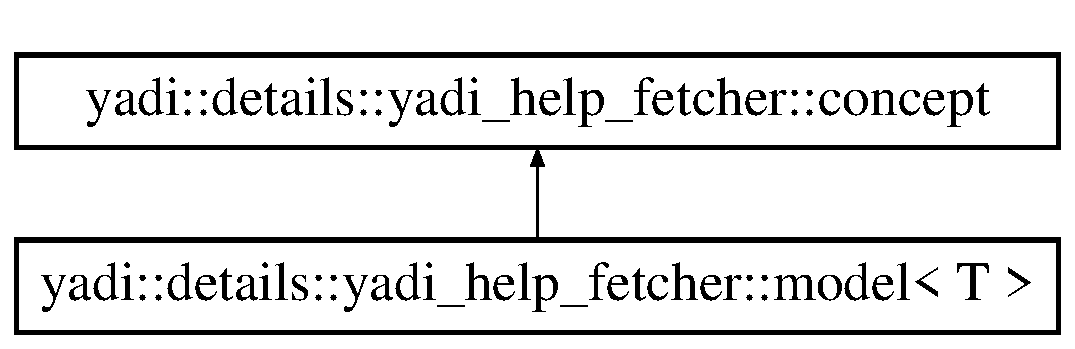
\includegraphics[height=2.000000cm]{structyadi_1_1details_1_1yadi__help__fetcher_1_1concept}
\end{center}
\end{figure}
\subsection*{Public Member Functions}
\begin{DoxyCompactItemize}
\item 
\mbox{\Hypertarget{structyadi_1_1details_1_1yadi__help__fetcher_1_1concept_ae1dab24d74d79eb7b385509d5628b402}\label{structyadi_1_1details_1_1yadi__help__fetcher_1_1concept_ae1dab24d74d79eb7b385509d5628b402}} 
virtual std\+::string {\bfseries get\+Help} (std\+::string const \&type) const =0
\item 
\mbox{\Hypertarget{structyadi_1_1details_1_1yadi__help__fetcher_1_1concept_ac61809b7604489e5176a2d0f8ad3e776}\label{structyadi_1_1details_1_1yadi__help__fetcher_1_1concept_ac61809b7604489e5176a2d0f8ad3e776}} 
virtual std\+::vector$<$ std\+::string $>$ {\bfseries get\+Types} () const =0
\item 
\mbox{\Hypertarget{structyadi_1_1details_1_1yadi__help__fetcher_1_1concept_a2d55ab2f5201a53381743ffc59119057}\label{structyadi_1_1details_1_1yadi__help__fetcher_1_1concept_a2d55ab2f5201a53381743ffc59119057}} 
virtual std\+::unique\+\_\+ptr$<$ \hyperlink{structyadi_1_1details_1_1yadi__help__fetcher_1_1concept}{concept} $>$ {\bfseries clone} () const =0
\end{DoxyCompactItemize}


The documentation for this struct was generated from the following file\+:\begin{DoxyCompactItemize}
\item 
src/yadi/details/help.\+hpp\end{DoxyCompactItemize}

\hypertarget{structyadi_1_1details_1_1ctr__helper}{}\section{yadi\+:\+:details\+:\+:ctr\+\_\+helper$<$ BT, IT, bool $>$ Struct Template Reference}
\label{structyadi_1_1details_1_1ctr__helper}\index{yadi\+::details\+::ctr\+\_\+helper$<$ B\+T, I\+T, bool $>$@{yadi\+::details\+::ctr\+\_\+helper$<$ B\+T, I\+T, bool $>$}}


\subsection{Detailed Description}
\subsubsection*{template$<$typename BT, typename IT, bool = meta\+::is\+\_\+by\+\_\+value$<$\+B\+T$>$\+::value$>$\newline
struct yadi\+::details\+::ctr\+\_\+helper$<$ B\+T, I\+T, bool $>$}



Definition at line 167 of file initializers.\+hpp.



The documentation for this struct was generated from the following file\+:\begin{DoxyCompactItemize}
\item 
src/yadi/details/initializers.\+hpp\end{DoxyCompactItemize}

\hypertarget{structyadi_1_1details_1_1ctr__helper_3_01_b_t_00_01_i_t_00_01false_01_4}{}\section{yadi\+:\+:details\+:\+:ctr\+\_\+helper$<$ BT, IT, false $>$ Struct Template Reference}
\label{structyadi_1_1details_1_1ctr__helper_3_01_b_t_00_01_i_t_00_01false_01_4}\index{yadi\+::details\+::ctr\+\_\+helper$<$ B\+T, I\+T, false $>$@{yadi\+::details\+::ctr\+\_\+helper$<$ B\+T, I\+T, false $>$}}
\subsection*{Static Public Member Functions}
\begin{DoxyCompactItemize}
\item 
\mbox{\Hypertarget{structyadi_1_1details_1_1ctr__helper_3_01_b_t_00_01_i_t_00_01false_01_4_a4a2cfcc0cdaa40eeccc054b8b5fc5dcd}\label{structyadi_1_1details_1_1ctr__helper_3_01_b_t_00_01_i_t_00_01false_01_4_a4a2cfcc0cdaa40eeccc054b8b5fc5dcd}} 
{\footnotesize template$<$typename... A\+R\+GS$>$ }\\static \hyperlink{namespaceyadi_a92290eb27cd90666aa87b17d854af9fe}{ptr\+\_\+type\+\_\+t}$<$ BT $>$ {\bfseries init} (A\+R\+G\+S... args)
\end{DoxyCompactItemize}


\subsection{Detailed Description}
\subsubsection*{template$<$typename BT, typename IT$>$\newline
struct yadi\+::details\+::ctr\+\_\+helper$<$ B\+T, I\+T, false $>$}



Definition at line 180 of file initializers.\+hpp.



The documentation for this struct was generated from the following file\+:\begin{DoxyCompactItemize}
\item 
src/yadi/details/initializers.\+hpp\end{DoxyCompactItemize}

\hypertarget{structyadi_1_1details_1_1ctr__helper_3_01_b_t_00_01_i_t_00_01true_01_4}{}\section{yadi\+:\+:details\+:\+:ctr\+\_\+helper$<$ BT, IT, true $>$ Struct Template Reference}
\label{structyadi_1_1details_1_1ctr__helper_3_01_b_t_00_01_i_t_00_01true_01_4}\index{yadi\+::details\+::ctr\+\_\+helper$<$ B\+T, I\+T, true $>$@{yadi\+::details\+::ctr\+\_\+helper$<$ B\+T, I\+T, true $>$}}
\subsection*{Static Public Member Functions}
\begin{DoxyCompactItemize}
\item 
\mbox{\Hypertarget{structyadi_1_1details_1_1ctr__helper_3_01_b_t_00_01_i_t_00_01true_01_4_a3c5dce230474dd7c1299bee33f9745af}\label{structyadi_1_1details_1_1ctr__helper_3_01_b_t_00_01_i_t_00_01true_01_4_a3c5dce230474dd7c1299bee33f9745af}} 
{\footnotesize template$<$typename... A\+R\+GS$>$ }\\static \hyperlink{namespaceyadi_a92290eb27cd90666aa87b17d854af9fe}{ptr\+\_\+type\+\_\+t}$<$ BT $>$ {\bfseries init} (A\+R\+G\+S... args)
\end{DoxyCompactItemize}


\subsection{Detailed Description}
\subsubsection*{template$<$typename BT, typename IT$>$\newline
struct yadi\+::details\+::ctr\+\_\+helper$<$ B\+T, I\+T, true $>$}



Definition at line 170 of file initializers.\+hpp.



The documentation for this struct was generated from the following file\+:\begin{DoxyCompactItemize}
\item 
src/yadi/details/initializers.\+hpp\end{DoxyCompactItemize}

\hypertarget{structyadi_1_1meta_1_1derive__base__type}{}\section{yadi\+:\+:meta\+:\+:derive\+\_\+base\+\_\+type$<$ T $>$ Struct Template Reference}
\label{structyadi_1_1meta_1_1derive__base__type}\index{yadi\+::meta\+::derive\+\_\+base\+\_\+type$<$ T $>$@{yadi\+::meta\+::derive\+\_\+base\+\_\+type$<$ T $>$}}


{\ttfamily \#include $<$type\+\_\+utils.\+hpp$>$}

\subsection*{Public Types}
\begin{DoxyCompactItemize}
\item 
\mbox{\Hypertarget{structyadi_1_1meta_1_1derive__base__type_a90b70b03e448a160fab74a151cd871a5}\label{structyadi_1_1meta_1_1derive__base__type_a90b70b03e448a160fab74a151cd871a5}} 
using {\bfseries base\+\_\+type} = bare\+\_\+t$<$ T $>$
\end{DoxyCompactItemize}


\subsection{Detailed Description}
\subsubsection*{template$<$typename T$>$\newline
struct yadi\+::meta\+::derive\+\_\+base\+\_\+type$<$ T $>$}

For type T, provide the factory base type that creates T. For example, for T std\+::unique\+\_\+ptr$<$int$>$, int would be the base type. 
\begin{DoxyTemplParams}{Template Parameters}
{\em T} & \\
\hline
\end{DoxyTemplParams}


Definition at line 51 of file type\+\_\+utils.\+hpp.



The documentation for this struct was generated from the following file\+:\begin{DoxyCompactItemize}
\item 
src/yadi/details/type\+\_\+utils.\+hpp\end{DoxyCompactItemize}

\hypertarget{structyadi_1_1factory}{}\section{yadi\+:\+:factory$<$ BT $>$ Struct Template Reference}
\label{structyadi_1_1factory}\index{yadi\+::factory$<$ B\+T $>$@{yadi\+::factory$<$ B\+T $>$}}
\subsection*{Classes}
\begin{DoxyCompactItemize}
\item 
struct \hyperlink{structyadi_1_1factory_1_1yadi__info}{yadi\+\_\+info}
\end{DoxyCompactItemize}
\subsection*{Public Types}
\begin{DoxyCompactItemize}
\item 
\mbox{\Hypertarget{structyadi_1_1factory_aa53aaa7d106c458d492e767d39c93369}\label{structyadi_1_1factory_aa53aaa7d106c458d492e767d39c93369}} 
using {\bfseries base\+\_\+type} = BT
\item 
\mbox{\Hypertarget{structyadi_1_1factory_abda283c5fcd47651b797b8f2dd29a122}\label{structyadi_1_1factory_abda283c5fcd47651b797b8f2dd29a122}} 
using {\bfseries initializer\+\_\+type} = std\+::function$<$ \hyperlink{namespaceyadi_a92290eb27cd90666aa87b17d854af9fe}{ptr\+\_\+type\+\_\+t}$<$ base\+\_\+type $>$(Y\+A\+M\+L\+::\+Node)$>$
\item 
\mbox{\Hypertarget{structyadi_1_1factory_a6e477a43b3072583702cc388e8028b47}\label{structyadi_1_1factory_a6e477a43b3072583702cc388e8028b47}} 
using {\bfseries ptr\+\_\+type} = \hyperlink{namespaceyadi_a92290eb27cd90666aa87b17d854af9fe}{ptr\+\_\+type\+\_\+t}$<$ base\+\_\+type $>$
\item 
\mbox{\Hypertarget{structyadi_1_1factory_a4d95d91a535e999a61357303812130b2}\label{structyadi_1_1factory_a4d95d91a535e999a61357303812130b2}} 
using {\bfseries type\+\_\+store} = std\+::map$<$ std\+::string, \hyperlink{structyadi_1_1factory_1_1yadi__info}{yadi\+\_\+info} $>$
\end{DoxyCompactItemize}
\subsection*{Static Public Member Functions}
\begin{DoxyCompactItemize}
\item 
static void \hyperlink{structyadi_1_1factory_a512c17ea9ca1bde8dec81c22b08e5278}{register\+\_\+type} (std\+::string type, \hyperlink{structyadi_1_1factory_1_1yadi__info}{yadi\+\_\+info} yadis)
\begin{DoxyCompactList}\small\item\em Registers initializer to type. When create is called with type this initializer will be called. Overwrites initializer if already registered (will change). \end{DoxyCompactList}\item 
static ptr\+\_\+type \hyperlink{structyadi_1_1factory_a600474900d2c6fa5d09935a641298bd5}{create} (std\+::string const \&type, Y\+A\+M\+L\+::\+Node const \&config=\{\})
\begin{DoxyCompactList}\small\item\em Calls the initializer associated with type passing the given Y\+A\+ML config. \end{DoxyCompactList}\item 
static type\+\_\+store const  \& \hyperlink{structyadi_1_1factory_aa167d70b963561d24c8a32f680d7e8c0}{types} ()
\begin{DoxyCompactList}\small\item\em Stored types and their registered initializers and help. \end{DoxyCompactList}\end{DoxyCompactItemize}


\subsection{Member Function Documentation}
\mbox{\Hypertarget{structyadi_1_1factory_a600474900d2c6fa5d09935a641298bd5}\label{structyadi_1_1factory_a600474900d2c6fa5d09935a641298bd5}} 
\index{yadi\+::factory@{yadi\+::factory}!create@{create}}
\index{create@{create}!yadi\+::factory@{yadi\+::factory}}
\subsubsection{\texorpdfstring{create()}{create()}}
{\footnotesize\ttfamily template$<$typename BT $>$ \\
\hyperlink{structyadi_1_1factory}{factory}$<$ BT $>$\+::ptr\+\_\+type \hyperlink{structyadi_1_1factory}{yadi\+::factory}$<$ BT $>$\+::create (\begin{DoxyParamCaption}\item[{std\+::string const \&}]{type,  }\item[{Y\+A\+M\+L\+::\+Node const \&}]{config = {\ttfamily \{\}} }\end{DoxyParamCaption})\hspace{0.3cm}{\ttfamily [static]}}



Calls the initializer associated with type passing the given Y\+A\+ML config. 


\begin{DoxyParams}{Parameters}
{\em type} & \\
\hline
{\em config} & \\
\hline
\end{DoxyParams}
\begin{DoxyReturn}{Returns}
The result of the registered initializer 
\end{DoxyReturn}

\begin{DoxyExceptions}{Exceptions}
{\em std\+::runtime\+\_\+error} & if no initializer is registered for type \\
\hline
\end{DoxyExceptions}
\mbox{\Hypertarget{structyadi_1_1factory_a512c17ea9ca1bde8dec81c22b08e5278}\label{structyadi_1_1factory_a512c17ea9ca1bde8dec81c22b08e5278}} 
\index{yadi\+::factory@{yadi\+::factory}!register\+\_\+type@{register\+\_\+type}}
\index{register\+\_\+type@{register\+\_\+type}!yadi\+::factory@{yadi\+::factory}}
\subsubsection{\texorpdfstring{register\+\_\+type()}{register\_type()}}
{\footnotesize\ttfamily template$<$typename BT $>$ \\
void \hyperlink{structyadi_1_1factory}{yadi\+::factory}$<$ BT $>$\+::register\+\_\+type (\begin{DoxyParamCaption}\item[{std\+::string}]{type,  }\item[{\hyperlink{structyadi_1_1factory_1_1yadi__info}{yadi\+\_\+info}}]{yadis }\end{DoxyParamCaption})\hspace{0.3cm}{\ttfamily [static]}}



Registers initializer to type. When create is called with type this initializer will be called. Overwrites initializer if already registered (will change). 


\begin{DoxyParams}{Parameters}
{\em type} & \\
\hline
{\em initializer} & \\
\hline
\end{DoxyParams}
\mbox{\Hypertarget{structyadi_1_1factory_aa167d70b963561d24c8a32f680d7e8c0}\label{structyadi_1_1factory_aa167d70b963561d24c8a32f680d7e8c0}} 
\index{yadi\+::factory@{yadi\+::factory}!types@{types}}
\index{types@{types}!yadi\+::factory@{yadi\+::factory}}
\subsubsection{\texorpdfstring{types()}{types()}}
{\footnotesize\ttfamily template$<$typename BT $>$ \\
\hyperlink{structyadi_1_1factory}{factory}$<$ BT $>$\+::type\+\_\+store const  \& \hyperlink{structyadi_1_1factory}{yadi\+::factory}$<$ BT $>$\+::types (\begin{DoxyParamCaption}{ }\end{DoxyParamCaption})\hspace{0.3cm}{\ttfamily [static]}}



Stored types and their registered initializers and help. 

\begin{DoxyReturn}{Returns}

\end{DoxyReturn}


The documentation for this struct was generated from the following file\+:\begin{DoxyCompactItemize}
\item 
src/yadi/details/factory.\+hpp\end{DoxyCompactItemize}

\hypertarget{structyadi_1_1factory__traits}{}\section{yadi\+:\+:factory\+\_\+traits$<$ BT $>$ Struct Template Reference}
\label{structyadi_1_1factory__traits}\index{yadi\+::factory\+\_\+traits$<$ B\+T $>$@{yadi\+::factory\+\_\+traits$<$ B\+T $>$}}


Factory traits that can be changed for BT.  




{\ttfamily \#include $<$factory.\+hpp$>$}

\subsection*{Public Types}
\begin{DoxyCompactItemize}
\item 
\mbox{\Hypertarget{structyadi_1_1factory__traits_a9a3b539941324b3aef58464863c76b55}\label{structyadi_1_1factory__traits_a9a3b539941324b3aef58464863c76b55}} 
using {\bfseries ptr\+\_\+type} = std\+::unique\+\_\+ptr$<$ BT $>$
\end{DoxyCompactItemize}
\subsection*{Static Public Attributes}
\begin{DoxyCompactItemize}
\item 
\mbox{\Hypertarget{structyadi_1_1factory__traits_af63ff1e85feaa7a1215130ac4d63e308}\label{structyadi_1_1factory__traits_af63ff1e85feaa7a1215130ac4d63e308}} 
static const bool \hyperlink{structyadi_1_1factory__traits_af63ff1e85feaa7a1215130ac4d63e308}{direct\+\_\+from\+\_\+yaml} = false
\begin{DoxyCompactList}\small\item\em The type of pointer to return from create. \end{DoxyCompactList}\end{DoxyCompactItemize}


\subsection{Detailed Description}
\subsubsection*{template$<$typename BT$>$\newline
struct yadi\+::factory\+\_\+traits$<$ B\+T $>$}

Factory traits that can be changed for BT. 


\begin{DoxyTemplParams}{Template Parameters}
{\em BT} & \\
\hline
\end{DoxyTemplParams}


Definition at line 66 of file factory.\+hpp.



The documentation for this struct was generated from the following file\+:\begin{DoxyCompactItemize}
\item 
src/yadi/details/factory.\+hpp\end{DoxyCompactItemize}

\hypertarget{structyadi_1_1details_1_1function__call__via__yaml}{}\section{yadi\+:\+:details\+:\+:function\+\_\+call\+\_\+via\+\_\+yaml$<$ T $>$ Struct Template Reference}
\label{structyadi_1_1details_1_1function__call__via__yaml}\index{yadi\+::details\+::function\+\_\+call\+\_\+via\+\_\+yaml$<$ T $>$@{yadi\+::details\+::function\+\_\+call\+\_\+via\+\_\+yaml$<$ T $>$}}
\subsection*{Public Types}
\begin{DoxyCompactItemize}
\item 
\mbox{\Hypertarget{structyadi_1_1details_1_1function__call__via__yaml_afaa3b21dcbc0e1a15738d1b6d2aa01d0}\label{structyadi_1_1details_1_1function__call__via__yaml_afaa3b21dcbc0e1a15738d1b6d2aa01d0}} 
using {\bfseries result\+\_\+type} = function\+\_\+traits\+\_\+result\+\_\+type$<$ T $>$
\item 
\mbox{\Hypertarget{structyadi_1_1details_1_1function__call__via__yaml_a2e36b4fa05d0394972a9f45f06d7ab05}\label{structyadi_1_1details_1_1function__call__via__yaml_a2e36b4fa05d0394972a9f45f06d7ab05}} 
using {\bfseries params\+\_\+type} = function\+\_\+traits\+\_\+params\+\_\+type$<$ T $>$
\item 
\mbox{\Hypertarget{structyadi_1_1details_1_1function__call__via__yaml_a81a291cb5024c27cd93a3853b47a265b}\label{structyadi_1_1details_1_1function__call__via__yaml_a81a291cb5024c27cd93a3853b47a265b}} 
using {\bfseries function\+\_\+type} = function\+\_\+traits\+\_\+function\+\_\+type$<$ T $>$
\item 
\mbox{\Hypertarget{structyadi_1_1details_1_1function__call__via__yaml_a63df821b6a02c14851dabbddd3dd18a0}\label{structyadi_1_1details_1_1function__call__via__yaml_a63df821b6a02c14851dabbddd3dd18a0}} 
using {\bfseries index\+\_\+sequence} = function\+\_\+traits\+\_\+index\+\_\+sequence$<$ T $>$
\end{DoxyCompactItemize}
\subsection*{Static Public Member Functions}
\begin{DoxyCompactItemize}
\item 
\mbox{\Hypertarget{structyadi_1_1details_1_1function__call__via__yaml_a811aa6a0b4643bbf95384e108635e459}\label{structyadi_1_1details_1_1function__call__via__yaml_a811aa6a0b4643bbf95384e108635e459}} 
static result\+\_\+type {\bfseries call} (function\+\_\+type func, Y\+A\+M\+L\+::\+Node const \&yaml)
\end{DoxyCompactItemize}


\subsection{Detailed Description}
\subsubsection*{template$<$typename T$>$\newline
struct yadi\+::details\+::function\+\_\+call\+\_\+via\+\_\+yaml$<$ T $>$}



Definition at line 254 of file initializers.\+hpp.



The documentation for this struct was generated from the following file\+:\begin{DoxyCompactItemize}
\item 
src/yadi/details/initializers.\+hpp\end{DoxyCompactItemize}

\hypertarget{structyadi_1_1details_1_1function__traits}{}\section{yadi\+:\+:details\+:\+:function\+\_\+traits$<$ T $>$ Struct Template Reference}
\label{structyadi_1_1details_1_1function__traits}\index{yadi\+::details\+::function\+\_\+traits$<$ T $>$@{yadi\+::details\+::function\+\_\+traits$<$ T $>$}}


\subsection{Detailed Description}
\subsubsection*{template$<$typename T$>$\newline
struct yadi\+::details\+::function\+\_\+traits$<$ T $>$}



Definition at line 223 of file initializers.\+hpp.



The documentation for this struct was generated from the following file\+:\begin{DoxyCompactItemize}
\item 
src/yadi/details/initializers.\+hpp\end{DoxyCompactItemize}

\hypertarget{structyadi_1_1details_1_1function__traits_3_01_r_07_5_08_07_args_8_8_8_08_4}{}\section{yadi\+:\+:details\+:\+:function\+\_\+traits$<$ R($\ast$)(Args...)$>$ Struct Template Reference}
\label{structyadi_1_1details_1_1function__traits_3_01_r_07_5_08_07_args_8_8_8_08_4}\index{yadi\+::details\+::function\+\_\+traits$<$ R($\ast$)(\+Args...)$>$@{yadi\+::details\+::function\+\_\+traits$<$ R($\ast$)(\+Args...)$>$}}
\subsection*{Public Types}
\begin{DoxyCompactItemize}
\item 
\mbox{\Hypertarget{structyadi_1_1details_1_1function__traits_3_01_r_07_5_08_07_args_8_8_8_08_4_aaa153c66f8001956278b60d9596283ff}\label{structyadi_1_1details_1_1function__traits_3_01_r_07_5_08_07_args_8_8_8_08_4_aaa153c66f8001956278b60d9596283ff}} 
using {\bfseries result\+\_\+type} = R
\item 
\mbox{\Hypertarget{structyadi_1_1details_1_1function__traits_3_01_r_07_5_08_07_args_8_8_8_08_4_a4a8d56109e247e39be130228d361d626}\label{structyadi_1_1details_1_1function__traits_3_01_r_07_5_08_07_args_8_8_8_08_4_a4a8d56109e247e39be130228d361d626}} 
using {\bfseries params\+\_\+type} = std\+::tuple$<$ meta\+::bare\+\_\+t$<$ Args $>$... $>$
\item 
\mbox{\Hypertarget{structyadi_1_1details_1_1function__traits_3_01_r_07_5_08_07_args_8_8_8_08_4_a2b9f01eb0463dada8e25dd6d6e5abbe1}\label{structyadi_1_1details_1_1function__traits_3_01_r_07_5_08_07_args_8_8_8_08_4_a2b9f01eb0463dada8e25dd6d6e5abbe1}} 
using {\bfseries function\+\_\+type} = std\+::function$<$ R(Args...)$>$
\item 
\mbox{\Hypertarget{structyadi_1_1details_1_1function__traits_3_01_r_07_5_08_07_args_8_8_8_08_4_a8443ef70c4af55cf7eb50b8698fbd3d3}\label{structyadi_1_1details_1_1function__traits_3_01_r_07_5_08_07_args_8_8_8_08_4_a8443ef70c4af55cf7eb50b8698fbd3d3}} 
using {\bfseries index\+\_\+sequence} = std\+::index\+\_\+sequence\+\_\+for$<$ Args... $>$
\end{DoxyCompactItemize}


\subsection{Detailed Description}
\subsubsection*{template$<$typename R, typename... Args$>$\newline
struct yadi\+::details\+::function\+\_\+traits$<$ R($\ast$)(\+Args...)$>$}



Definition at line 226 of file initializers.\+hpp.



The documentation for this struct was generated from the following file\+:\begin{DoxyCompactItemize}
\item 
src/yadi/details/initializers.\+hpp\end{DoxyCompactItemize}

\hypertarget{structyadi_1_1details_1_1function__traits_3_01std_1_1function_3_01_r_07_args_8_8_8_08_4_01_4}{}\section{yadi\+:\+:details\+:\+:function\+\_\+traits$<$ std\+:\+:function$<$ R(Args...)$>$ $>$ Struct Template Reference}
\label{structyadi_1_1details_1_1function__traits_3_01std_1_1function_3_01_r_07_args_8_8_8_08_4_01_4}\index{yadi\+::details\+::function\+\_\+traits$<$ std\+::function$<$ R(\+Args...)$>$ $>$@{yadi\+::details\+::function\+\_\+traits$<$ std\+::function$<$ R(\+Args...)$>$ $>$}}
\subsection*{Public Types}
\begin{DoxyCompactItemize}
\item 
\mbox{\Hypertarget{structyadi_1_1details_1_1function__traits_3_01std_1_1function_3_01_r_07_args_8_8_8_08_4_01_4_ac068b05439b1192cd569fa36f2dfc27a}\label{structyadi_1_1details_1_1function__traits_3_01std_1_1function_3_01_r_07_args_8_8_8_08_4_01_4_ac068b05439b1192cd569fa36f2dfc27a}} 
using {\bfseries result\+\_\+type} = R
\item 
\mbox{\Hypertarget{structyadi_1_1details_1_1function__traits_3_01std_1_1function_3_01_r_07_args_8_8_8_08_4_01_4_a3f7c503ebb6e36d7dfabb9f172fa45a3}\label{structyadi_1_1details_1_1function__traits_3_01std_1_1function_3_01_r_07_args_8_8_8_08_4_01_4_a3f7c503ebb6e36d7dfabb9f172fa45a3}} 
using {\bfseries params\+\_\+type} = std\+::tuple$<$ meta\+::bare\+\_\+t$<$ Args $>$... $>$
\item 
\mbox{\Hypertarget{structyadi_1_1details_1_1function__traits_3_01std_1_1function_3_01_r_07_args_8_8_8_08_4_01_4_a736c672a78223b1be22be46ed7910c78}\label{structyadi_1_1details_1_1function__traits_3_01std_1_1function_3_01_r_07_args_8_8_8_08_4_01_4_a736c672a78223b1be22be46ed7910c78}} 
using {\bfseries function\+\_\+type} = std\+::function$<$ R(Args...)$>$
\item 
\mbox{\Hypertarget{structyadi_1_1details_1_1function__traits_3_01std_1_1function_3_01_r_07_args_8_8_8_08_4_01_4_ada4af304d47ba359182ee23002f372e1}\label{structyadi_1_1details_1_1function__traits_3_01std_1_1function_3_01_r_07_args_8_8_8_08_4_01_4_ada4af304d47ba359182ee23002f372e1}} 
using {\bfseries index\+\_\+sequence} = std\+::index\+\_\+sequence\+\_\+for$<$ Args... $>$
\end{DoxyCompactItemize}


\subsection{Detailed Description}
\subsubsection*{template$<$typename R, typename... Args$>$\newline
struct yadi\+::details\+::function\+\_\+traits$<$ std\+::function$<$ R(\+Args...)$>$ $>$}



Definition at line 234 of file initializers.\+hpp.



The documentation for this struct was generated from the following file\+:\begin{DoxyCompactItemize}
\item 
src/yadi/details/initializers.\+hpp\end{DoxyCompactItemize}

\hypertarget{structyadi_1_1meta_1_1if__convertible__then}{}\section{yadi\+:\+:meta\+:\+:if\+\_\+convertible\+\_\+then$<$ L, R, RT, typename $>$ Struct Template Reference}
\label{structyadi_1_1meta_1_1if__convertible__then}\index{yadi\+::meta\+::if\+\_\+convertible\+\_\+then$<$ L, R, R\+T, typename $>$@{yadi\+::meta\+::if\+\_\+convertible\+\_\+then$<$ L, R, R\+T, typename $>$}}


{\ttfamily \#include $<$type\+\_\+utils.\+hpp$>$}

\subsection*{Public Types}
\begin{DoxyCompactItemize}
\item 
\mbox{\Hypertarget{structyadi_1_1meta_1_1if__convertible__then_af5f58c3e86c8f9a05a918090e86d618f}\label{structyadi_1_1meta_1_1if__convertible__then_af5f58c3e86c8f9a05a918090e86d618f}} 
using {\bfseries type} = RT
\end{DoxyCompactItemize}


\subsection{Detailed Description}
\subsubsection*{template$<$typename L, typename R, typename RT, typename = typename std\+::enable\+\_\+if$<$std\+::is\+\_\+convertible$<$\+L, R$>$\+::value$>$\+::type$>$\newline
struct yadi\+::meta\+::if\+\_\+convertible\+\_\+then$<$ L, R, R\+T, typename $>$}

If lest is same as right then provide type\+\_\+type as type. 
\begin{DoxyTemplParams}{Template Parameters}
{\em L} & left \\
\hline
{\em R} & right \\
\hline
{\em RT} & result type \\
\hline
\end{DoxyTemplParams}


Definition at line 29 of file type\+\_\+utils.\+hpp.



The documentation for this struct was generated from the following file\+:\begin{DoxyCompactItemize}
\item 
src/yadi/details/type\+\_\+utils.\+hpp\end{DoxyCompactItemize}

\hypertarget{structyadi_1_1details_1_1init__no__arg__helper}{}\section{yadi\+:\+:details\+:\+:init\+\_\+no\+\_\+arg\+\_\+helper$<$ BT, IT, by\+\_\+value $>$ Struct Template Reference}
\label{structyadi_1_1details_1_1init__no__arg__helper}\index{yadi\+::details\+::init\+\_\+no\+\_\+arg\+\_\+helper$<$ B\+T, I\+T, by\+\_\+value $>$@{yadi\+::details\+::init\+\_\+no\+\_\+arg\+\_\+helper$<$ B\+T, I\+T, by\+\_\+value $>$}}


\subsection{Detailed Description}
\subsubsection*{template$<$typename BT, typename IT, bool by\+\_\+value = meta\+::is\+\_\+by\+\_\+value$<$\+B\+T$>$\+::value$>$\newline
struct yadi\+::details\+::init\+\_\+no\+\_\+arg\+\_\+helper$<$ B\+T, I\+T, by\+\_\+value $>$}



Definition at line 147 of file initializers.\+hpp.



The documentation for this struct was generated from the following file\+:\begin{DoxyCompactItemize}
\item 
src/yadi/details/initializers.\+hpp\end{DoxyCompactItemize}

\hypertarget{structyadi_1_1details_1_1init__no__arg__helper_3_01_b_t_00_01_i_t_00_01false_01_4}{}\section{yadi\+:\+:details\+:\+:init\+\_\+no\+\_\+arg\+\_\+helper$<$ BT, IT, false $>$ Struct Template Reference}
\label{structyadi_1_1details_1_1init__no__arg__helper_3_01_b_t_00_01_i_t_00_01false_01_4}\index{yadi\+::details\+::init\+\_\+no\+\_\+arg\+\_\+helper$<$ B\+T, I\+T, false $>$@{yadi\+::details\+::init\+\_\+no\+\_\+arg\+\_\+helper$<$ B\+T, I\+T, false $>$}}
\subsection*{Static Public Member Functions}
\begin{DoxyCompactItemize}
\item 
\mbox{\Hypertarget{structyadi_1_1details_1_1init__no__arg__helper_3_01_b_t_00_01_i_t_00_01false_01_4_a43b81409264cbd054bab2f66a886c47b}\label{structyadi_1_1details_1_1init__no__arg__helper_3_01_b_t_00_01_i_t_00_01false_01_4_a43b81409264cbd054bab2f66a886c47b}} 
static \hyperlink{namespaceyadi_a92290eb27cd90666aa87b17d854af9fe}{ptr\+\_\+type\+\_\+t}$<$ BT $>$ {\bfseries init} ()
\end{DoxyCompactItemize}


The documentation for this struct was generated from the following file\+:\begin{DoxyCompactItemize}
\item 
src/yadi/details/initializers.\+hpp\end{DoxyCompactItemize}

\hypertarget{structyadi_1_1details_1_1init__no__arg__helper_3_01_b_t_00_01_i_t_00_01true_01_4}{}\section{yadi\+:\+:details\+:\+:init\+\_\+no\+\_\+arg\+\_\+helper$<$ BT, IT, true $>$ Struct Template Reference}
\label{structyadi_1_1details_1_1init__no__arg__helper_3_01_b_t_00_01_i_t_00_01true_01_4}\index{yadi\+::details\+::init\+\_\+no\+\_\+arg\+\_\+helper$<$ B\+T, I\+T, true $>$@{yadi\+::details\+::init\+\_\+no\+\_\+arg\+\_\+helper$<$ B\+T, I\+T, true $>$}}
\subsection*{Static Public Member Functions}
\begin{DoxyCompactItemize}
\item 
\mbox{\Hypertarget{structyadi_1_1details_1_1init__no__arg__helper_3_01_b_t_00_01_i_t_00_01true_01_4_a12f7dde0d08a746a0b4855b6009bbb40}\label{structyadi_1_1details_1_1init__no__arg__helper_3_01_b_t_00_01_i_t_00_01true_01_4_a12f7dde0d08a746a0b4855b6009bbb40}} 
static \hyperlink{namespaceyadi_a92290eb27cd90666aa87b17d854af9fe}{ptr\+\_\+type\+\_\+t}$<$ BT $>$ {\bfseries init} ()
\end{DoxyCompactItemize}


\subsection{Detailed Description}
\subsubsection*{template$<$typename BT, typename IT$>$\newline
struct yadi\+::details\+::init\+\_\+no\+\_\+arg\+\_\+helper$<$ B\+T, I\+T, true $>$}



Definition at line 158 of file initializers.\+hpp.



The documentation for this struct was generated from the following file\+:\begin{DoxyCompactItemize}
\item 
src/yadi/details/initializers.\+hpp\end{DoxyCompactItemize}

\hypertarget{structyadi_1_1details_1_1init__yaml__helper}{}\section{yadi\+:\+:details\+:\+:init\+\_\+yaml\+\_\+helper$<$ BT, IT, by\+\_\+value $>$ Struct Template Reference}
\label{structyadi_1_1details_1_1init__yaml__helper}\index{yadi\+::details\+::init\+\_\+yaml\+\_\+helper$<$ B\+T, I\+T, by\+\_\+value $>$@{yadi\+::details\+::init\+\_\+yaml\+\_\+helper$<$ B\+T, I\+T, by\+\_\+value $>$}}


\subsection{Detailed Description}
\subsubsection*{template$<$typename BT, typename IT, bool by\+\_\+value = meta\+::is\+\_\+by\+\_\+value$<$\+B\+T$>$\+::value$>$\newline
struct yadi\+::details\+::init\+\_\+yaml\+\_\+helper$<$ B\+T, I\+T, by\+\_\+value $>$}



Definition at line 127 of file initializers.\+hpp.



The documentation for this struct was generated from the following file\+:\begin{DoxyCompactItemize}
\item 
src/yadi/details/initializers.\+hpp\end{DoxyCompactItemize}

\hypertarget{structyadi_1_1details_1_1init__yaml__helper_3_01_b_t_00_01_i_t_00_01false_01_4}{}\section{yadi\+:\+:details\+:\+:init\+\_\+yaml\+\_\+helper$<$ BT, IT, false $>$ Struct Template Reference}
\label{structyadi_1_1details_1_1init__yaml__helper_3_01_b_t_00_01_i_t_00_01false_01_4}\index{yadi\+::details\+::init\+\_\+yaml\+\_\+helper$<$ B\+T, I\+T, false $>$@{yadi\+::details\+::init\+\_\+yaml\+\_\+helper$<$ B\+T, I\+T, false $>$}}
\subsection*{Static Public Member Functions}
\begin{DoxyCompactItemize}
\item 
\mbox{\Hypertarget{structyadi_1_1details_1_1init__yaml__helper_3_01_b_t_00_01_i_t_00_01false_01_4_a056433bd33067957aba92754dbe1f3a2}\label{structyadi_1_1details_1_1init__yaml__helper_3_01_b_t_00_01_i_t_00_01false_01_4_a056433bd33067957aba92754dbe1f3a2}} 
static \hyperlink{namespaceyadi_a92290eb27cd90666aa87b17d854af9fe}{ptr\+\_\+type\+\_\+t}$<$ BT $>$ {\bfseries init} (Y\+A\+M\+L\+::\+Node const \&config)
\end{DoxyCompactItemize}


The documentation for this struct was generated from the following file\+:\begin{DoxyCompactItemize}
\item 
src/yadi/details/initializers.\+hpp\end{DoxyCompactItemize}

\hypertarget{structyadi_1_1details_1_1init__yaml__helper_3_01_b_t_00_01_i_t_00_01true_01_4}{}\section{yadi\+:\+:details\+:\+:init\+\_\+yaml\+\_\+helper$<$ BT, IT, true $>$ Struct Template Reference}
\label{structyadi_1_1details_1_1init__yaml__helper_3_01_b_t_00_01_i_t_00_01true_01_4}\index{yadi\+::details\+::init\+\_\+yaml\+\_\+helper$<$ B\+T, I\+T, true $>$@{yadi\+::details\+::init\+\_\+yaml\+\_\+helper$<$ B\+T, I\+T, true $>$}}
\subsection*{Static Public Member Functions}
\begin{DoxyCompactItemize}
\item 
\mbox{\Hypertarget{structyadi_1_1details_1_1init__yaml__helper_3_01_b_t_00_01_i_t_00_01true_01_4_a7070e4a34e5dea1bd2388e45f67430c9}\label{structyadi_1_1details_1_1init__yaml__helper_3_01_b_t_00_01_i_t_00_01true_01_4_a7070e4a34e5dea1bd2388e45f67430c9}} 
static \hyperlink{namespaceyadi_a92290eb27cd90666aa87b17d854af9fe}{ptr\+\_\+type\+\_\+t}$<$ BT $>$ {\bfseries init} (Y\+A\+M\+L\+::\+Node const \&config)
\end{DoxyCompactItemize}


The documentation for this struct was generated from the following file\+:\begin{DoxyCompactItemize}
\item 
src/yadi/details/initializers.\+hpp\end{DoxyCompactItemize}

\hypertarget{structyadi_1_1meta_1_1is__by__value}{}\section{yadi\+:\+:meta\+:\+:is\+\_\+by\+\_\+value$<$ BT $>$ Struct Template Reference}
\label{structyadi_1_1meta_1_1is__by__value}\index{yadi\+::meta\+::is\+\_\+by\+\_\+value$<$ B\+T $>$@{yadi\+::meta\+::is\+\_\+by\+\_\+value$<$ B\+T $>$}}


Determine is factory returns by value.  




{\ttfamily \#include $<$type\+\_\+utils.\+hpp$>$}

\subsection*{Static Public Attributes}
\begin{DoxyCompactItemize}
\item 
\mbox{\Hypertarget{structyadi_1_1meta_1_1is__by__value_a430929d9f810b08e62a35550240aa925}\label{structyadi_1_1meta_1_1is__by__value_a430929d9f810b08e62a35550240aa925}} 
static const bool {\bfseries value} = std\+::is\+\_\+same$<$BT, \hyperlink{namespaceyadi_a92290eb27cd90666aa87b17d854af9fe}{ptr\+\_\+type\+\_\+t}$<$BT$>$$>$\+::value
\end{DoxyCompactItemize}


\subsection{Detailed Description}
\subsubsection*{template$<$typename BT$>$\newline
struct yadi\+::meta\+::is\+\_\+by\+\_\+value$<$ B\+T $>$}

Determine is factory returns by value. 


\begin{DoxyTemplParams}{Template Parameters}
{\em BT} & \\
\hline
\end{DoxyTemplParams}


Definition at line 41 of file type\+\_\+utils.\+hpp.



The documentation for this struct was generated from the following file\+:\begin{DoxyCompactItemize}
\item 
src/yadi/details/type\+\_\+utils.\+hpp\end{DoxyCompactItemize}

\hypertarget{structyadi_1_1details_1_1yadi__help__fetcher_1_1model}{}\section{yadi\+:\+:details\+:\+:yadi\+\_\+help\+\_\+fetcher\+:\+:model$<$ T $>$ Struct Template Reference}
\label{structyadi_1_1details_1_1yadi__help__fetcher_1_1model}\index{yadi\+::details\+::yadi\+\_\+help\+\_\+fetcher\+::model$<$ T $>$@{yadi\+::details\+::yadi\+\_\+help\+\_\+fetcher\+::model$<$ T $>$}}
Inheritance diagram for yadi\+:\+:details\+:\+:yadi\+\_\+help\+\_\+fetcher\+:\+:model$<$ T $>$\+:\begin{figure}[H]
\begin{center}
\leavevmode
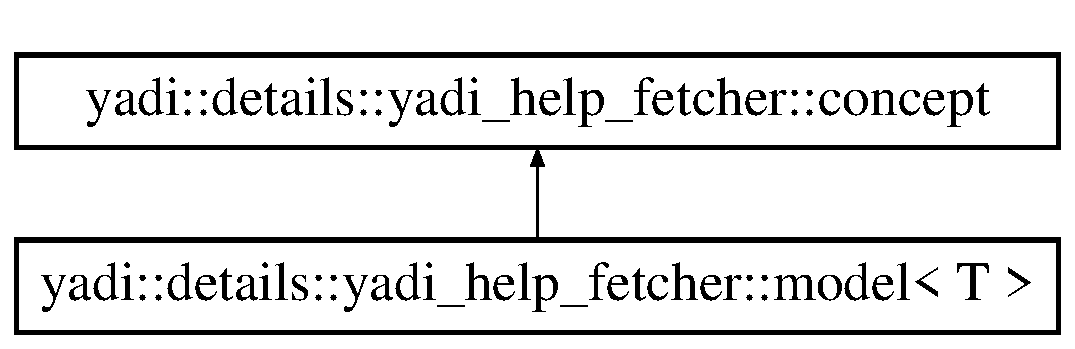
\includegraphics[height=2.000000cm]{structyadi_1_1details_1_1yadi__help__fetcher_1_1model}
\end{center}
\end{figure}
\subsection*{Public Member Functions}
\begin{DoxyCompactItemize}
\item 
\mbox{\Hypertarget{structyadi_1_1details_1_1yadi__help__fetcher_1_1model_ae7febad4b673cc9087c1c5db808f45ab}\label{structyadi_1_1details_1_1yadi__help__fetcher_1_1model_ae7febad4b673cc9087c1c5db808f45ab}} 
{\bfseries model} (T const \&types)
\item 
\mbox{\Hypertarget{structyadi_1_1details_1_1yadi__help__fetcher_1_1model_a9d821dcf2fbd773b39920b78df593a04}\label{structyadi_1_1details_1_1yadi__help__fetcher_1_1model_a9d821dcf2fbd773b39920b78df593a04}} 
std\+::string {\bfseries get\+Help} (std\+::string const \&type) const override
\item 
\mbox{\Hypertarget{structyadi_1_1details_1_1yadi__help__fetcher_1_1model_ae399334faaece23170abfe1b88b640f1}\label{structyadi_1_1details_1_1yadi__help__fetcher_1_1model_ae399334faaece23170abfe1b88b640f1}} 
std\+::vector$<$ std\+::string $>$ {\bfseries get\+Types} () const override
\item 
\mbox{\Hypertarget{structyadi_1_1details_1_1yadi__help__fetcher_1_1model_a75b6ce0c4e310bbfb9ff5f508f480094}\label{structyadi_1_1details_1_1yadi__help__fetcher_1_1model_a75b6ce0c4e310bbfb9ff5f508f480094}} 
std\+::unique\+\_\+ptr$<$ \hyperlink{structyadi_1_1details_1_1yadi__help__fetcher_1_1concept}{concept} $>$ {\bfseries clone} () const override
\end{DoxyCompactItemize}
\subsection*{Public Attributes}
\begin{DoxyCompactItemize}
\item 
\mbox{\Hypertarget{structyadi_1_1details_1_1yadi__help__fetcher_1_1model_a97e1055826d47be6fff465c2be501173}\label{structyadi_1_1details_1_1yadi__help__fetcher_1_1model_a97e1055826d47be6fff465c2be501173}} 
T const  \& {\bfseries types}
\end{DoxyCompactItemize}


The documentation for this struct was generated from the following file\+:\begin{DoxyCompactItemize}
\item 
src/yadi/details/help.\+hpp\end{DoxyCompactItemize}

\hypertarget{structyadi_1_1yadi__help}{}\section{yadi\+:\+:yadi\+\_\+help Struct Reference}
\label{structyadi_1_1yadi__help}\index{yadi\+::yadi\+\_\+help@{yadi\+::yadi\+\_\+help}}
\subsection*{Public Types}
\begin{DoxyCompactItemize}
\item 
\mbox{\Hypertarget{structyadi_1_1yadi__help_a3f208166dac982fc5ea2da59cccfd51e}\label{structyadi_1_1yadi__help_a3f208166dac982fc5ea2da59cccfd51e}} 
using {\bfseries help\+\_\+store} = std\+::map$<$ std\+::string, \hyperlink{structyadi_1_1details_1_1yadi__help__fetcher}{details\+::yadi\+\_\+help\+\_\+fetcher} $>$
\item 
\mbox{\Hypertarget{structyadi_1_1yadi__help_aaa85b3a9116a8dd35a91db333576bf59}\label{structyadi_1_1yadi__help_aaa85b3a9116a8dd35a91db333576bf59}} 
using {\bfseries name\+\_\+store} = std\+::map$<$ std\+::type\+\_\+index, std\+::string $>$
\end{DoxyCompactItemize}
\subsection*{Static Public Member Functions}
\begin{DoxyCompactItemize}
\item 
\mbox{\Hypertarget{structyadi_1_1yadi__help_add1c3496248cd02834c8bd835d4ac417}\label{structyadi_1_1yadi__help_add1c3496248cd02834c8bd835d4ac417}} 
{\footnotesize template$<$typename BT , typename TS $>$ }\\static void {\bfseries register\+\_\+factory} (std\+::string name, TS const \&types)
\item 
\mbox{\Hypertarget{structyadi_1_1yadi__help_ade91b0fb56b72ee34c7e3be193faac02}\label{structyadi_1_1yadi__help_ade91b0fb56b72ee34c7e3be193faac02}} 
{\footnotesize template$<$typename BT $>$ }\\static bool {\bfseries has\+\_\+name} ()
\item 
\mbox{\Hypertarget{structyadi_1_1yadi__help_a106e37c78f02730ba7d54f9892932ede}\label{structyadi_1_1yadi__help_a106e37c78f02730ba7d54f9892932ede}} 
{\footnotesize template$<$typename BT $>$ }\\static std\+::string {\bfseries get\+\_\+name} ()
\item 
\mbox{\Hypertarget{structyadi_1_1yadi__help_a9ddef20988be744f132c45009a4c3810}\label{structyadi_1_1yadi__help_a9ddef20988be744f132c45009a4c3810}} 
static help\+\_\+store const  \& {\bfseries helps} ()
\item 
\mbox{\Hypertarget{structyadi_1_1yadi__help_a41fb4a566cae38f7530d1c9f08f72a8f}\label{structyadi_1_1yadi__help_a41fb4a566cae38f7530d1c9f08f72a8f}} 
static name\+\_\+store const  \& {\bfseries names} ()
\end{DoxyCompactItemize}


The documentation for this struct was generated from the following files\+:\begin{DoxyCompactItemize}
\item 
src/yadi/details/help.\+hpp\item 
src/yadi/details/help.\+cpp\end{DoxyCompactItemize}

\hypertarget{structyadi_1_1details_1_1yadi__help__fetcher}{}\section{yadi\+:\+:details\+:\+:yadi\+\_\+help\+\_\+fetcher Struct Reference}
\label{structyadi_1_1details_1_1yadi__help__fetcher}\index{yadi\+::details\+::yadi\+\_\+help\+\_\+fetcher@{yadi\+::details\+::yadi\+\_\+help\+\_\+fetcher}}
\subsection*{Classes}
\begin{DoxyCompactItemize}
\item 
struct \hyperlink{structyadi_1_1details_1_1yadi__help__fetcher_1_1concept}{concept}
\item 
struct \hyperlink{structyadi_1_1details_1_1yadi__help__fetcher_1_1model}{model}
\end{DoxyCompactItemize}
\subsection*{Public Member Functions}
\begin{DoxyCompactItemize}
\item 
\mbox{\Hypertarget{structyadi_1_1details_1_1yadi__help__fetcher_a5f8b1e45b37c8aa71ddfefeeaf8d05bf}\label{structyadi_1_1details_1_1yadi__help__fetcher_a5f8b1e45b37c8aa71ddfefeeaf8d05bf}} 
{\bfseries yadi\+\_\+help\+\_\+fetcher} (\hyperlink{structyadi_1_1details_1_1yadi__help__fetcher}{yadi\+\_\+help\+\_\+fetcher} const \&other)
\item 
\mbox{\Hypertarget{structyadi_1_1details_1_1yadi__help__fetcher_a0d919e20c92d45110827975ae7127f5f}\label{structyadi_1_1details_1_1yadi__help__fetcher_a0d919e20c92d45110827975ae7127f5f}} 
{\footnotesize template$<$typename Y $>$ }\\{\bfseries yadi\+\_\+help\+\_\+fetcher} (Y const \&types)
\item 
\mbox{\Hypertarget{structyadi_1_1details_1_1yadi__help__fetcher_a74c236f0e49bd623a75b49ca3dbd201a}\label{structyadi_1_1details_1_1yadi__help__fetcher_a74c236f0e49bd623a75b49ca3dbd201a}} 
\hyperlink{structyadi_1_1details_1_1yadi__help__fetcher}{yadi\+\_\+help\+\_\+fetcher} \& {\bfseries operator=} (\hyperlink{structyadi_1_1details_1_1yadi__help__fetcher}{yadi\+\_\+help\+\_\+fetcher} const \&other)
\item 
\mbox{\Hypertarget{structyadi_1_1details_1_1yadi__help__fetcher_a16119e731cb7fcb5775ed36a570fefa5}\label{structyadi_1_1details_1_1yadi__help__fetcher_a16119e731cb7fcb5775ed36a570fefa5}} 
std\+::string {\bfseries get\+\_\+help} (std\+::string const \&type) const
\item 
\mbox{\Hypertarget{structyadi_1_1details_1_1yadi__help__fetcher_a5170a74f42bd371aa9eb40871d793478}\label{structyadi_1_1details_1_1yadi__help__fetcher_a5170a74f42bd371aa9eb40871d793478}} 
std\+::vector$<$ std\+::string $>$ {\bfseries get\+\_\+types} () const
\end{DoxyCompactItemize}


The documentation for this struct was generated from the following files\+:\begin{DoxyCompactItemize}
\item 
src/yadi/details/help.\+hpp\item 
src/yadi/details/help.\+cpp\end{DoxyCompactItemize}

\hypertarget{structyadi_1_1factory_1_1yadi__info}{}\section{yadi\+:\+:factory$<$ BT $>$\+:\+:yadi\+\_\+info Struct Reference}
\label{structyadi_1_1factory_1_1yadi__info}\index{yadi\+::factory$<$ B\+T $>$\+::yadi\+\_\+info@{yadi\+::factory$<$ B\+T $>$\+::yadi\+\_\+info}}
\subsection*{Public Attributes}
\begin{DoxyCompactItemize}
\item 
\mbox{\Hypertarget{structyadi_1_1factory_1_1yadi__info_a63c0e3eb9fd1e8051f5aacee3439c313}\label{structyadi_1_1factory_1_1yadi__info_a63c0e3eb9fd1e8051f5aacee3439c313}} 
initializer\+\_\+type {\bfseries initializer}
\item 
\mbox{\Hypertarget{structyadi_1_1factory_1_1yadi__info_a5b9a7705a796247d0049755236516015}\label{structyadi_1_1factory_1_1yadi__info_a5b9a7705a796247d0049755236516015}} 
std\+::string {\bfseries help}
\end{DoxyCompactItemize}


The documentation for this struct was generated from the following file\+:\begin{DoxyCompactItemize}
\item 
src/yadi/details/factory.\+hpp\end{DoxyCompactItemize}

\hypertarget{structyadi_1_1details_1_1yaml__to__tuple}{}\section{yadi\+:\+:details\+:\+:yaml\+\_\+to\+\_\+tuple$<$ tuple\+\_\+t, index $>$ Struct Template Reference}
\label{structyadi_1_1details_1_1yaml__to__tuple}\index{yadi\+::details\+::yaml\+\_\+to\+\_\+tuple$<$ tuple\+\_\+t, index $>$@{yadi\+::details\+::yaml\+\_\+to\+\_\+tuple$<$ tuple\+\_\+t, index $>$}}
\subsection*{Static Public Member Functions}
\begin{DoxyCompactItemize}
\item 
\mbox{\Hypertarget{structyadi_1_1details_1_1yaml__to__tuple_a0e0419b468a6df3f8f9427e1836d641c}\label{structyadi_1_1details_1_1yaml__to__tuple_a0e0419b468a6df3f8f9427e1836d641c}} 
static void {\bfseries to\+\_\+tuple} (tuple\+\_\+t \&out, Y\+A\+M\+L\+::\+Node const \&yaml)
\item 
\mbox{\Hypertarget{structyadi_1_1details_1_1yaml__to__tuple_ae25dd83334168cf48bf6bcf7d1c942c2}\label{structyadi_1_1details_1_1yaml__to__tuple_ae25dd83334168cf48bf6bcf7d1c942c2}} 
{\footnotesize template$<$typename arg\+\_\+type\+\_\+out $>$ }\\static void {\bfseries to\+\_\+arg\+\_\+types} (arg\+\_\+type\+\_\+out arg\+\_\+types)
\end{DoxyCompactItemize}


The documentation for this struct was generated from the following file\+:\begin{DoxyCompactItemize}
\item 
src/yadi/details/initializers.\+hpp\end{DoxyCompactItemize}

\hypertarget{structyadi_1_1details_1_1yaml__to__tuple_3_01tuple__t_00_010_01_4}{}\section{yadi\+:\+:details\+:\+:yaml\+\_\+to\+\_\+tuple$<$ tuple\+\_\+t, 0 $>$ Struct Template Reference}
\label{structyadi_1_1details_1_1yaml__to__tuple_3_01tuple__t_00_010_01_4}\index{yadi\+::details\+::yaml\+\_\+to\+\_\+tuple$<$ tuple\+\_\+t, 0 $>$@{yadi\+::details\+::yaml\+\_\+to\+\_\+tuple$<$ tuple\+\_\+t, 0 $>$}}
\subsection*{Static Public Member Functions}
\begin{DoxyCompactItemize}
\item 
\mbox{\Hypertarget{structyadi_1_1details_1_1yaml__to__tuple_3_01tuple__t_00_010_01_4_a5d8bce7dc03e42221c09af80cdef2ef5}\label{structyadi_1_1details_1_1yaml__to__tuple_3_01tuple__t_00_010_01_4_a5d8bce7dc03e42221c09af80cdef2ef5}} 
static void {\bfseries to\+\_\+tuple} (tuple\+\_\+t \&out, Y\+A\+M\+L\+::\+Node const \&yaml)
\item 
\mbox{\Hypertarget{structyadi_1_1details_1_1yaml__to__tuple_3_01tuple__t_00_010_01_4_a891c11157210a181cf92882730a9940e}\label{structyadi_1_1details_1_1yaml__to__tuple_3_01tuple__t_00_010_01_4_a891c11157210a181cf92882730a9940e}} 
{\footnotesize template$<$typename arg\+\_\+type\+\_\+out $>$ }\\static void {\bfseries to\+\_\+arg\+\_\+types} (arg\+\_\+type\+\_\+out arg\+\_\+types)
\end{DoxyCompactItemize}


The documentation for this struct was generated from the following file\+:\begin{DoxyCompactItemize}
\item 
src/yadi/details/initializers.\+hpp\end{DoxyCompactItemize}

%--- End generated contents ---

% Index
\backmatter
\newpage
\phantomsection
\clearemptydoublepage
\addcontentsline{toc}{chapter}{Index}
\printindex

\end{document}
